
\documentclass[12pt,a4paper,titlepage,listof=totoc,bibliography=totoc,chapteratlists=0pt]{scrreprt}

\begin{filecontents*}{\jobname.xmpdata}
	\Keywords{VR, IOT, TODO}
	\Title{Raspberry Poolüberwachung}
	\Author{Sebastian Egger}
\end{filecontents*}

\setcounter{tocdepth}{1}

\usepackage[utf8]{inputenc}
\usepackage[T1]{fontenc}
\usepackage{amsmath}
\usepackage{amsfonts}
\usepackage{amssymb}
\usepackage[table]{xcolor}
\usepackage{graphicx}
\usepackage[left=3.50cm, right=2.00cm, top=2.00cm, bottom=2.00cm,foot=1cm]{geometry}
\usepackage[splitrule,hang,flushmargin,multiple,bottom]{footmisc}
\usepackage{lmodern, textcomp}
\usepackage{lmodern}
\usepackage{pdfpages}
\usepackage[ngerman]{babel}
\usepackage{multicol}
\usepackage{subfig}
\usepackage{float}
\usepackage{array,tabularx,booktabs}
\usepackage{ragged2e}
\usepackage{lipsum}
\usepackage{wrapfig}

\newcolumntype{M}[1]{>{\centering\arraybackslash}m{#1}}

\usepackage{enumitem}
\newlist{compactitem}{itemize}{3}
\setlist[compactitem,1]{label=\textbullet, nosep,leftmargin=1.5em,labelwidth=*,align=left}
\setlist[compactitem,2]{label=--, nosep,leftmargin=1.5em,labelwidth=*,align=left}
\setlist[compactitem,3]{label=\textopenbullet, nosep,leftmargin=1.5em,labelwidth=*,align=left}
\newlist{compactenum}{enumerate}{3}
\setlist[compactenum,1]{label=\arabic*., nosep,leftmargin=1.5em,labelwidth=*,align=left}
\setlist[compactenum,2]{label=\alph*., nosep,leftmargin=1.5em,labelwidth=*,align=left}
\setlist[compactenum,3]{label=\roman*., nosep,leftmargin=1.5em,labelwidth=*,align=left}
\newlist{compactdesc}{description}{3}
\setlist[compactdesc]{leftmargin=1.5em,labelwidth=*,align=left}

\usepackage{microtype}

\usepackage[parfill]{parskip}

\definecolor{bluekeywords}{rgb}{0.13,0.13,1}
\definecolor{greencomments}{rgb}{0,0.5,0}
\definecolor{redstrings}{rgb}{0.9,0,0}
\definecolor{lightgray}{gray}{0.9}
\definecolor{lightblue}{rgb}{0.93,0.95,1.0}

\usepackage{listings}

\makeatletter
\lstdefinestyle{lststyle}{
	basicstyle=%
	\ttfamily
	\lst@ifdisplaystyle\scriptsize\fi
}
\makeatother

\renewcommand{\lstlistlistingname}{List of Listings}
% TODO: define other languages as needed
\lstset{
language=csh,
numbers=left,               
numberstyle=\tiny,          
showspaces=false,
showtabs=false,
breaklines=true,
lineskip=-1pt,
tabsize=2,
showstringspaces=false,
breakatwhitespace=true,
escapeinside={(*@}{@*)},
commentstyle=\color{greencomments},
keywordstyle=\color{bluekeywords}\bfseries,
stringstyle=\color{redstrings},
style=lststyle,
xleftmargin=17pt,
         framexleftmargin=17pt,
         framexrightmargin=5pt,
         framexbottommargin=4pt
}
\lstset{
morekeywords=
{abstract, event, new, struct,
as, explicit, null, switch,
base, extern, object, this,
bool, false, operator, throw,
break, finally, out, true,
byte, fixed, override, try,
case, float, params, typeof,
catch, for, private, uint,
char, foreach, protected, ulong,
checked, goto, public, unchecked,
class, if, readonly, unsafe,
const, implicit, ref, ushort,
continue, in, return, using,
decimal, int, sbyte, virtual,
default, interface, sealed, volatile,
delegate, internal, short, void,
do, is, sizeof, while,
double, lock, stackalloc,
else, long, static,
enum, namespace, string}
}
\lstdefinelanguage{TypeScript}{
	keywords={typeof, new, true, false, catch, function, return, null, switch, var, if, in, while, do, else, case, break, void, number, string, boolean, module, \$, export, for, this},
	keywordstyle=\color{blue}\bfseries,
	ndkeywords={class, export, boolean, throw, implements, import, this},
	ndkeywordstyle=\color{darkgray}\bfseries,
	identifierstyle=\color{black},
	sensitive=false,
	comment=[l]{//},
	morecomment=[s]{/*}{*/},
	commentstyle=\color{purple}\ttfamily,
	stringstyle=\color{red}\ttfamily,
	morestring=[b]',
	morestring=[b]"
}
\usepackage{caption}
\DeclareCaptionFont{white}{\color{white}}
\DeclareCaptionFormat{listing}{\colorbox[cmyk]{0.43, 0.35, 0.35,0.01}{\parbox{\textwidth}{\hspace{10pt}#1#2#3}}}
\captionsetup[lstlisting]{format=listing,labelfont=white,textfont=white} 
\captionsetup[table]{justification=centering, singlelinecheck=false}

\usepackage{setspace}
\newcommand{\MSonehalfspacing}{%
	\setstretch{1.44}%  default
	\ifcase \@ptsize \relax % 10pt
	\setstretch {1.448}%
	\or % 11pt
	\setstretch {1.399}%
	\or % 12pt
	\setstretch {1.433}%
	\fi
}

\newcommand{\setauthor}[1]{\ohead[]{#1}}

\usepackage[automark]{scrlayer-scrpage}
\pagestyle{scrheadings}
\automark{chapter}
\renewcommand\sectionmark[1]{\markright{\MakeMarkcase {\thesection\hskip .5em\relax#1}}}
\rohead{\ifnum\expandafter\pdfstrcmp\botmark=0 \rightmark\else\leftmark{} --- \rightmark\fi}
\ihead[]{\headmark}
\chead[]{}
\ohead{}
\cfoot[]{}
\ofoot[\pagemark]{\pagemark}
\setheadsepline{.1pt}

\usepackage[hyphens]{url}

\usepackage[a-1b]{pdfx}

\usepackage{hyperref}
\hypersetup{pdfa}

\usepackage[nonumberlist,toc,nopostdot]{glossaries}

\usepackage{chngcntr}
\counterwithout{footnote}{chapter}
\counterwithout{figure}{chapter}
\counterwithout{table}{chapter}
\AtBeginDocument{
	\counterwithout{lstlisting}{chapter}
	\urlstyle{sf}
}
\newcounter{RPages}

\makeatletter
\def\bstctlcite{\@ifnextchar[{\@bstctlcite}{\@bstctlcite[@auxout]}}
\def\@bstctlcite[#1]#2{\@bsphack
	\@for\@citeb:=#2\do{%
		\edef\@citeb{\expandafter\@firstofone\@citeb}%
		\if@filesw\immediate\write\csname #1\endcsname{\string\citation{\@citeb}}\fi}%
	\@esphack}
\makeatother

\clubpenalty=10000
\widowpenalty=10000
\displaywidowpenalty=10000
\interfootnotelinepenalty=10000

\title{Raspberry Poolüberwachung}
\author{Sebastian Egger, Florian Wilflingseder}

\makeindex
\makeglossaries
\begin{document}
\bstctlcite{IEEEexample:BSTcontrol}
\newcommand{\reminder}[1]
{ \textcolor{red}{<[{\bf\marginpar{\mbox{$<==$}} #1 }]>} }
\newcommand{\icode}[1]{\lstinline$#1$}
%\urlstyle{same}
%\setstretch{1.5}
\setstretch {1.433}
\renewcommand{\arraystretch}{1.2}

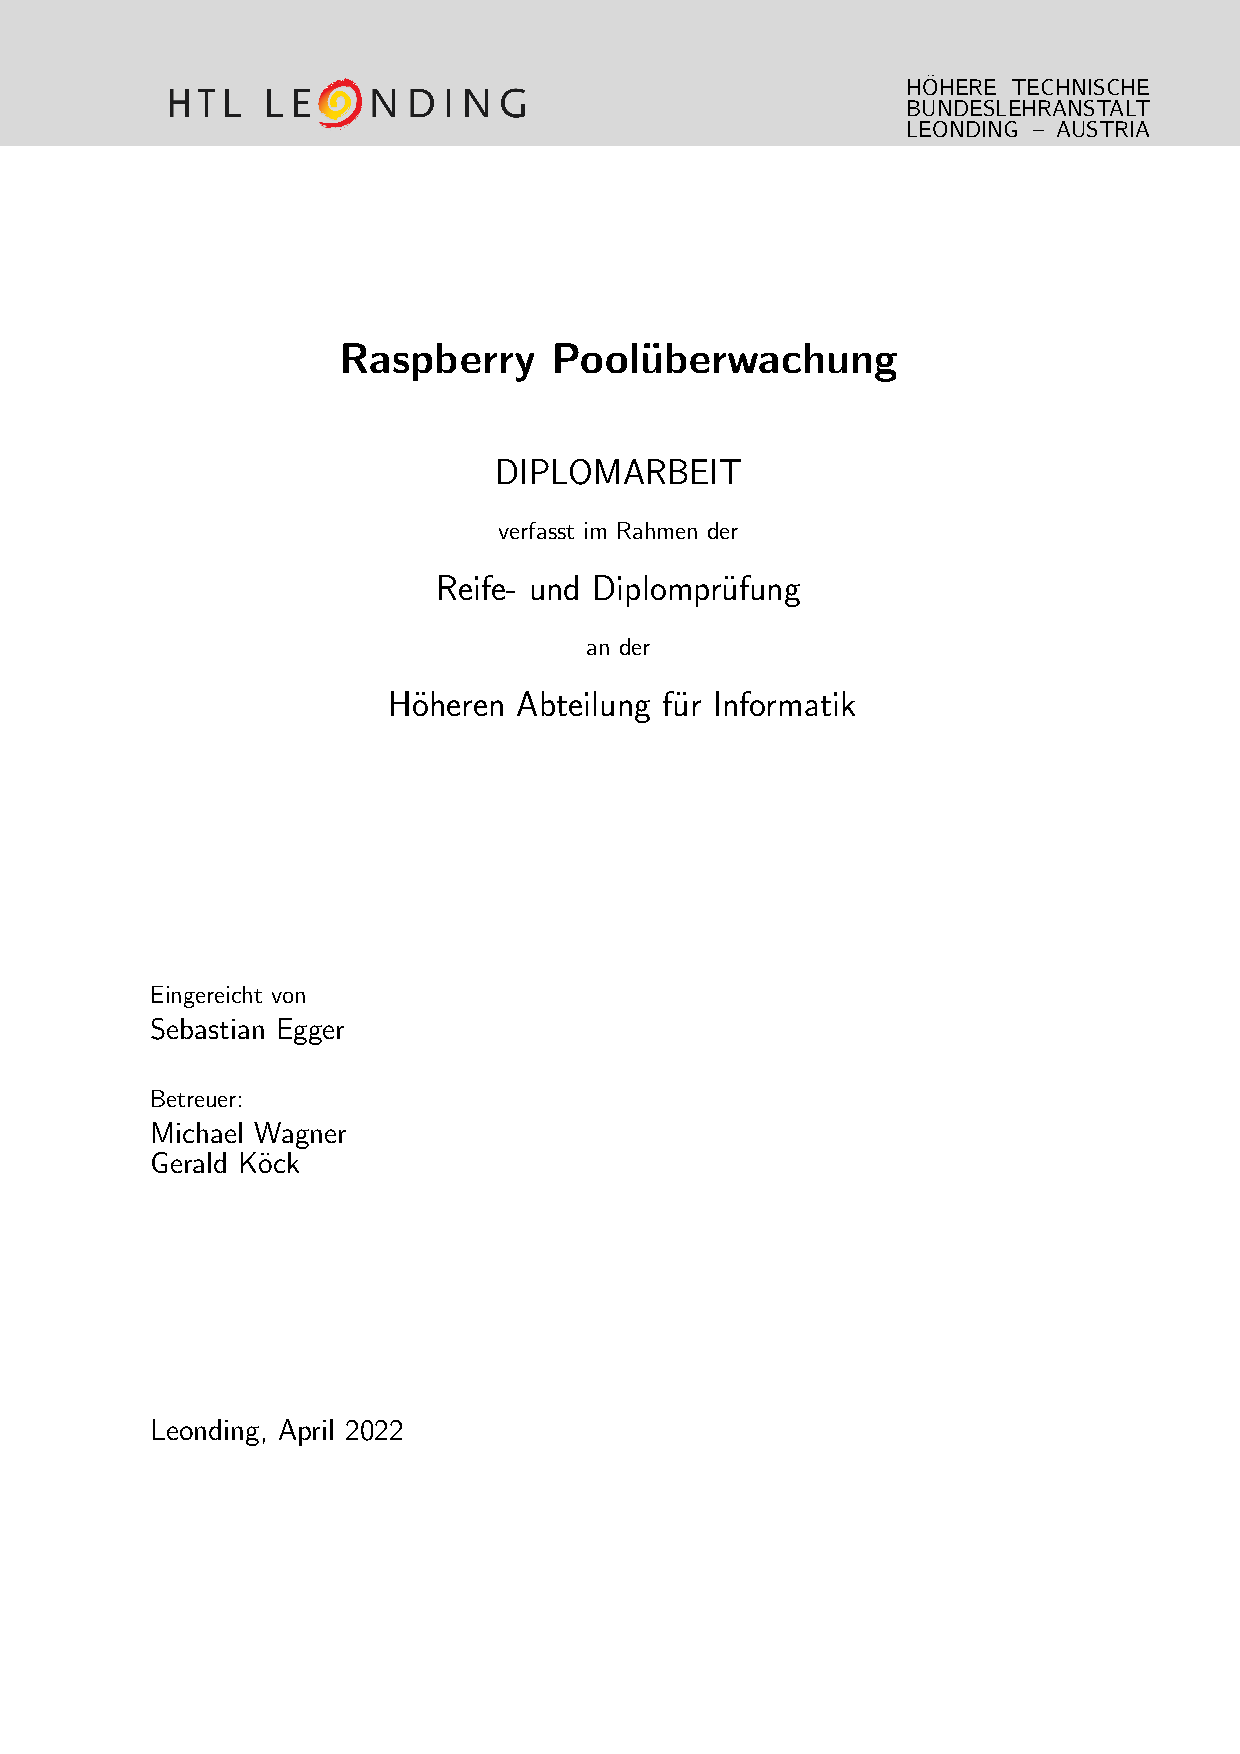
\includepdf{./titlepage/coversheet}
\pagenumbering{Roman}
\newpage
\thispagestyle{empty}
\vspace{3cm}
~ \\ \\
Ich erkläre an Eides statt, dass ich die vorliegende Diplomarbeit selbstständig und ohne fremde Hilfe verfasst, andere als die angegebenen Quellen und Hilfsmittel nicht benutzt bzw. die wörtlich oder sinngemäß entnommenen Stellen als solche kenntlich gemacht habe.

Die Arbeit wurde bisher in gleicher oder ähnlicher Weise keiner anderen Prüfungsbehörde vorgelegt und auch noch nicht veröffentlicht.

Die vorliegende Diplomarbeit ist mit dem elektronisch übermittelten Textdokument identisch.
\vspace{3cm}
% Hier kommt die Unterschrift drüber
\begin{tabbing}
Leonding, April 2022 \hspace{5cm} S. Egger \& F. Wilflingseder
\end{tabbing}
\vspace{10cm}
Zur Verbesserung der Lesbarkeit wurde in diesem Dokument auf eine geschlechtsneutrale Ausdrucksweise verzichtet.
Alle verwendeten Formulierungen richten sich jedoch an alle Geschlechter.
\newpage
\setcounter{page}{1}

\begin{spacing}{1}
    \chapter*{Zusammenfassung}
\end{spacing}
\begin{wrapfigure}{r}{0.3\textwidth}
    \begin{center}
      
\includegraphics[width=0.2\textwidth]{pics/question_mark.png}
    \end{center}
\end{wrapfigure}
Zusammenfassung unserer genialen Arbeit. Auf Deutsch.
Das ist das einzige Mal, dass eine Grafik in den Textfluss eingebunden wird.
Die gewählte Grafik soll irgendwie eure Arbeit repräsentieren.
Das ist ungewöhnlich für eine wissenschaftliche Arbeit aber eine Anforderung der Obrigkeit.
\emph{Bitte auf keinen Fall mit der Zusammenfassung verwechseln, die den Abschluss der Arbeit bildet!}



\pagestyle{plain}

\renewcommand{\lstlistlistingname}{Quellcodeverzeichnis}

\tableofcontents
\newpage
\setcounter{RPages}{\value{page}}
\setcounter{page}{0}
\pagenumbering{arabic}
\pagestyle{scrheadings}

\begin{spacing}{1}
\chapter{Einleitung}\label{chapter:introduction}
\end{spacing}
Unsere Diplomarbeit wurde in das Leben gerufen, um einen Pool überwachen zu können.
Aktuell sind mehrere Geräte für die Überwachung eines Pools erforderlich.
Ziel unserer Diplomarbeit ist es, die Funktionalitäten 
von einem Trübungssensor, Wellengangssensor und Temperatursensor zuverlässig in einem Gerät kosteneffizient zusammenzuführen 
und über ein UserInterface der Single Page Apllication einen 360 Grad Blick auf die Geschehnisse im Pool zu ermöglichen. 

\begin{spacing}{1}
\chapter{Umfeldanalyse}
\end{spacing}

Florian Wilflingseder

\begin{spacing}{1}
\chapter{Technologien}\label{chapter:tech}
\end{spacing}
\section{Raspberry Pi}
\setauthor{Sebastian Egger}

Das Projekt beinhaltet einen Raspberry Pi 4, welcher als MQTT Broker dient. Auf diesem Raspberry Pi läuft unser Backend mit DotNet, Docker und Samba.
Der Raspberry Pi hat 4 Gigabyte RAM und eine 32 Gigabyte SSD. 
Die Verbindung zwischen dem Raspberry und der SSD wird mit einem USB-Adapter hergestellt. 
Die SSD wurde unter dem Raspberry mittels einer Platine und Schrauben befestigt. 
Der Raspberry braucht mindestens 3 und maximal 11 Watt. 


\begin{figure}[H]
    \centering
    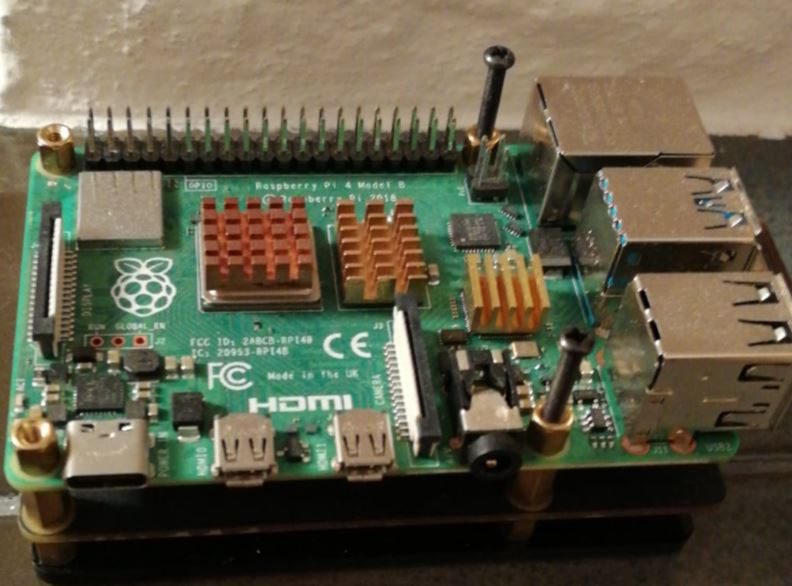
\includegraphics[width=1\textwidth]{pics/Raspberry.JPG}
    \caption{Raspberry Pi des Projektes}
\end{figure}

\subsection{Samba}
Der Raspberry dient weiters als File-Server. Für eine leichtere Datenübertragung zwischen Windows und Linux wird mit Hilfe von Samba über den Windows Explorer direkt auf den Raspberry Pi zugegriffen.
Somit können Files oder Projekte direkt von einem Laptop oder Computer auf den Raspberry PI gelegt werden.

\begin{figure}[H]
    \centering
    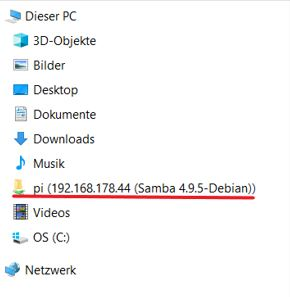
\includegraphics[width=0.5\textwidth]{pics/RaspberrySamba.JPG}
    \caption{Samba auf Laptop}
\end{figure}



\subsection {MQTT auf Raspberry Pi:}
Weiteres dient unser Raspberry auch als MQTT-Broker, welcher Messwerte von Sensoren empfängt und an das Backend, welches als MQTT-Client dient, übermittelt. 
Genaueres wie MQTT aufgebaut ist und in welcher Verbindung der MQTT-Broker zu den MQTT-Clients steht wird im Kapitel MQTT beschrieben.

\subsection {Installation und Verwendung von Docker auf dem Raspberry Pi:}

Docker ist eine Software, welche das Management von Containern übernimmt. Ein Container enthält alle Dateien, die zum Ausführen einer Software notwendig sind. 
Die Installation von Docker wird über ein Skript durchgeführt. 
Dieses wird direkt von Docker zur Verfügung gestellt und führt alle Schritte automatisch ohne weitere Eingaben vom Benutzer durch. 
Nach wenigen Minuten ist Docker betriebsbereit. 
Weiters ist auch eine zentralisierte Servicebereitstellungsplattform für containerisierte Apps 
mit dem Namen Portainer auf dem Raspberry Pi installiert, 
welche eine Liste aller Container und deren Informationen zur Verfügung stellt.
 


\subsection {Remote Access auf einen Raspberry PI:}
Bei Verwendung des Raspberry PI ohne direkt angeschlossenen Monitor kann mittels SSH (Secure Socket Shell) Protokoll von einem Laptop zugegriffen werden.
Dabei muss die IP-Adresse des Raspberry's im Netzwerk bekannt sein. WLAN-Router (FRITZ!Box) bieten über ihre standard IP-Adresse eine Übersicht der verbundenen Geräte, wo auch unter anderem der verbundene Raspberry Pi angezeigt wird. 

 \subsection{Was sind Ip-Adressen:}
Im oberen Kapitel Remote Access ist oft das Wort Ip-Adresse gefallen, deswegen wird in diesem Unterpunkt eine kleine Einführung über Ip-Adressen und Ihre Verwendung gegeben. 
Eine Ip-Adresse ist eine Adresse in Computernetzen, welche von einem Router vergeben wird.
 Einem Gerät kann maximal eine Ip-Adresse zugewiesen werden, jedoch kann die Ip-Adresse auch wechseln, wenn sich das Gerät zum Router erneut verbindet. 
 Im Router gibt es aber auch die Konfigurationsmöglichkeit, dass einem Gerät immer eine bestimmte Ip-Adresse zugewiesen wird. 






\section{MQTT}
\setauthor{Sebastian Egger}

\subsection{Was ist MQTT:}
MQTT ausgeschrieben Message Queuing  Telemetry Transport ist ein Protokoll, welches Nachrichten von einer Maschine zu einer anderen Maschine schickt. 
Ein MQTT Netzwerk besteht  aus mindestens einem MQTT-Broker und zwei MQTT-Clients. 
Wenn ein MQTT-Client eine Message an einen anderen MQTT-Client senden will, muss als erstes eine Message zu dem MQTT-Broker, welcher die Message zu einem sogenannten Topic zuweist, gesendet werden.
Ein Topic ist ein Bereich, wo bestimmte Nachrichten aufgelistet werden. 
Ein Topic in unserem Fall lautet mqtt/noice für den Noice-Sensor.  
Wenn ein oder mehrere MQTT-Clients diese Nachricht empfangen wollen, dann subscriben diese auf das Topic. 
Durch das subscriben von den Clients werden diese, sobald eine neue Message an das Topic gesendet wurde, benachrichtigt und können diese nun empfangen. 

\subsection {Verwendung von MQTT in unserem Projekt:}
Unser Projekt besteht aus 2 MQTT-Clients und 1 MQTT-Broker. 
Die Sensor Box ist ein MQTT-Client, welcher die Messwerte an den MQTT-Broker sendet. 
Der MQTT-Broker ist im Projekt der Raspberry PI. 
Zum Empfangen der Daten liest das Backend, welches den zweiten MQTT-Client darstellt, die Daten vom Raspberry ein.

\subsection{MQTT-Explorer:}
MQTT-Explorer ist eine kostenlose Software, welches sich für das Testen einer Connection zwischen MQTT-Client und Broker bestens eignet.
Der MQTT-Explorer ist ein weiterer MQTT-Client.
Zur Benutzung und Verbindung mit dem Raspberry ist ein Login mit der Ip-Adresse und Port des Brokers sowie dem dazugehörigen Benutzernamen und Passwort notwendig.

\begin{figure}[H]
    \centering
    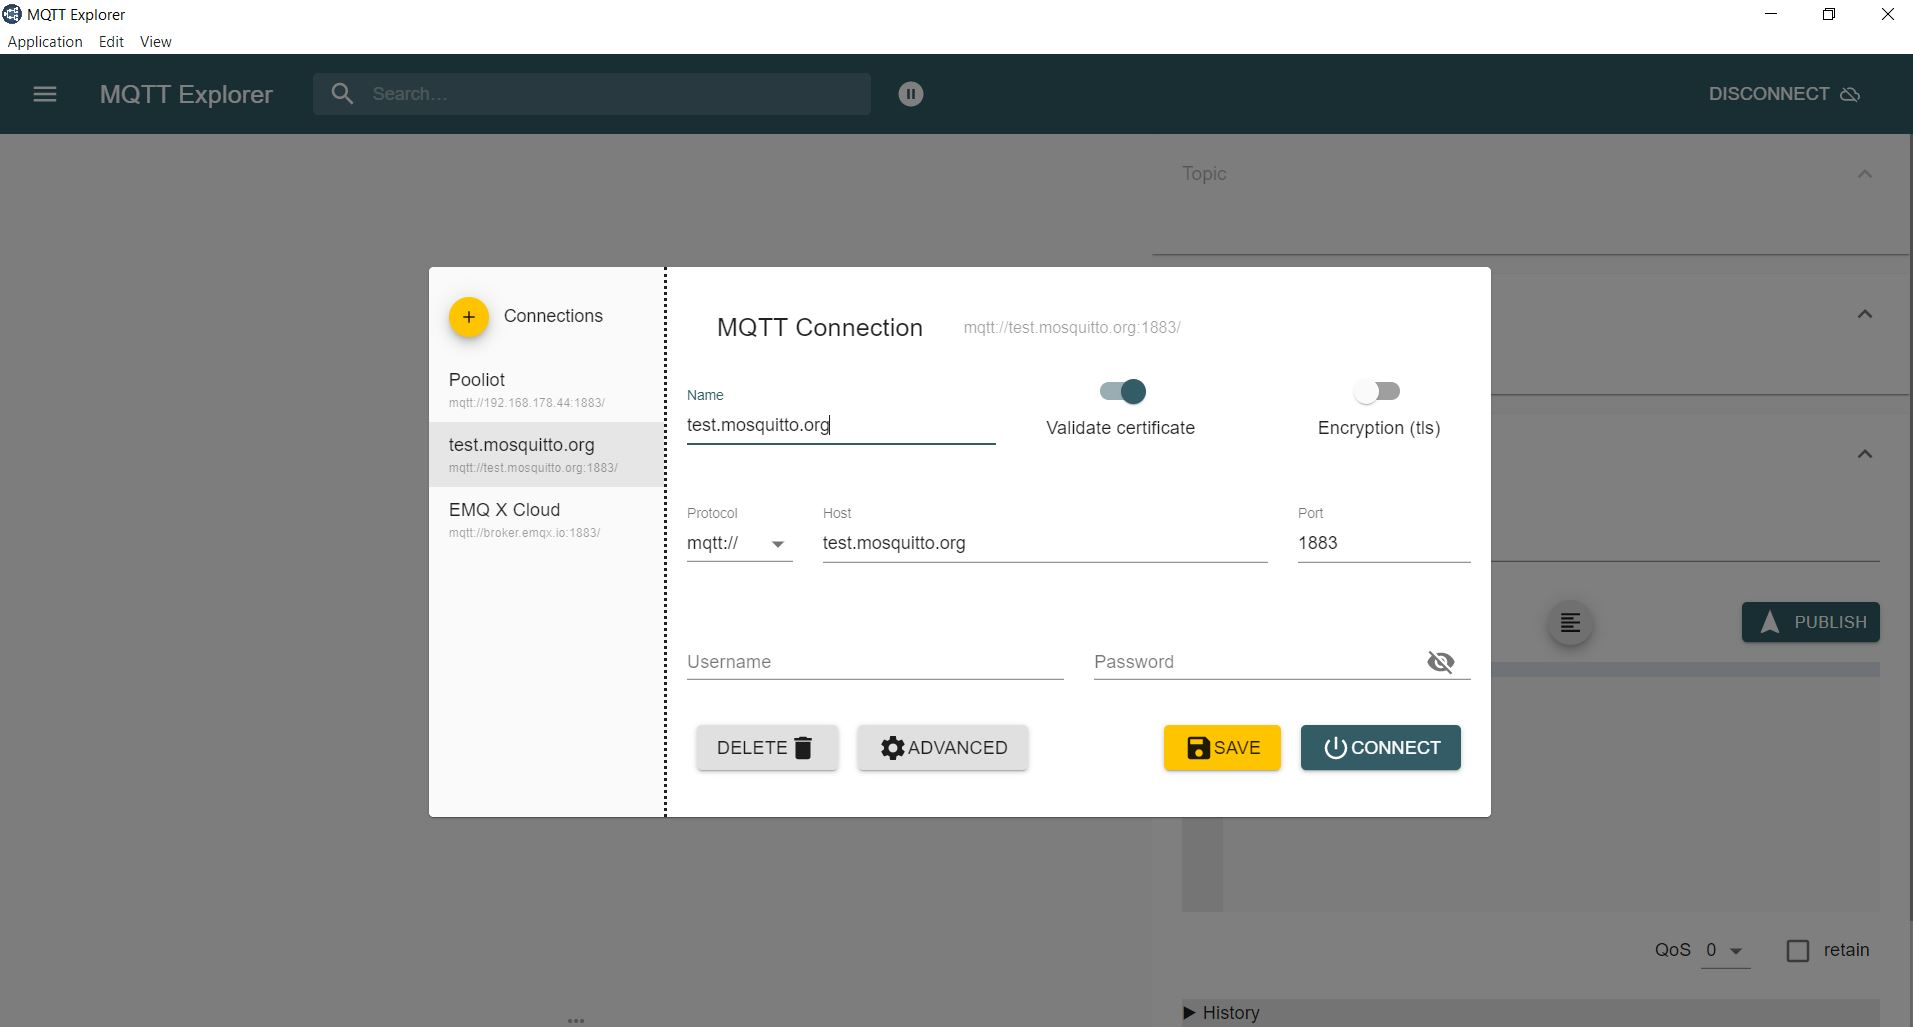
\includegraphics[width=1\textwidth]{pics/MQTTExplorerStartScreen.JPG}
    \caption{MQTT-Explorer Login}
\end{figure}


 Sobald eine Verbindung zu einem MQTT-Broker möglich ist, wird ein Screen mit dem Namen des Brokers und den dazugehörigen Topics aufgelistet. 
 In unten gezeigter Abbildung wurde eine Verbindung mit dem MQTT-Broker test.mosquitto.org hergestellt.  

 \begin{figure}[H]
    \centering
    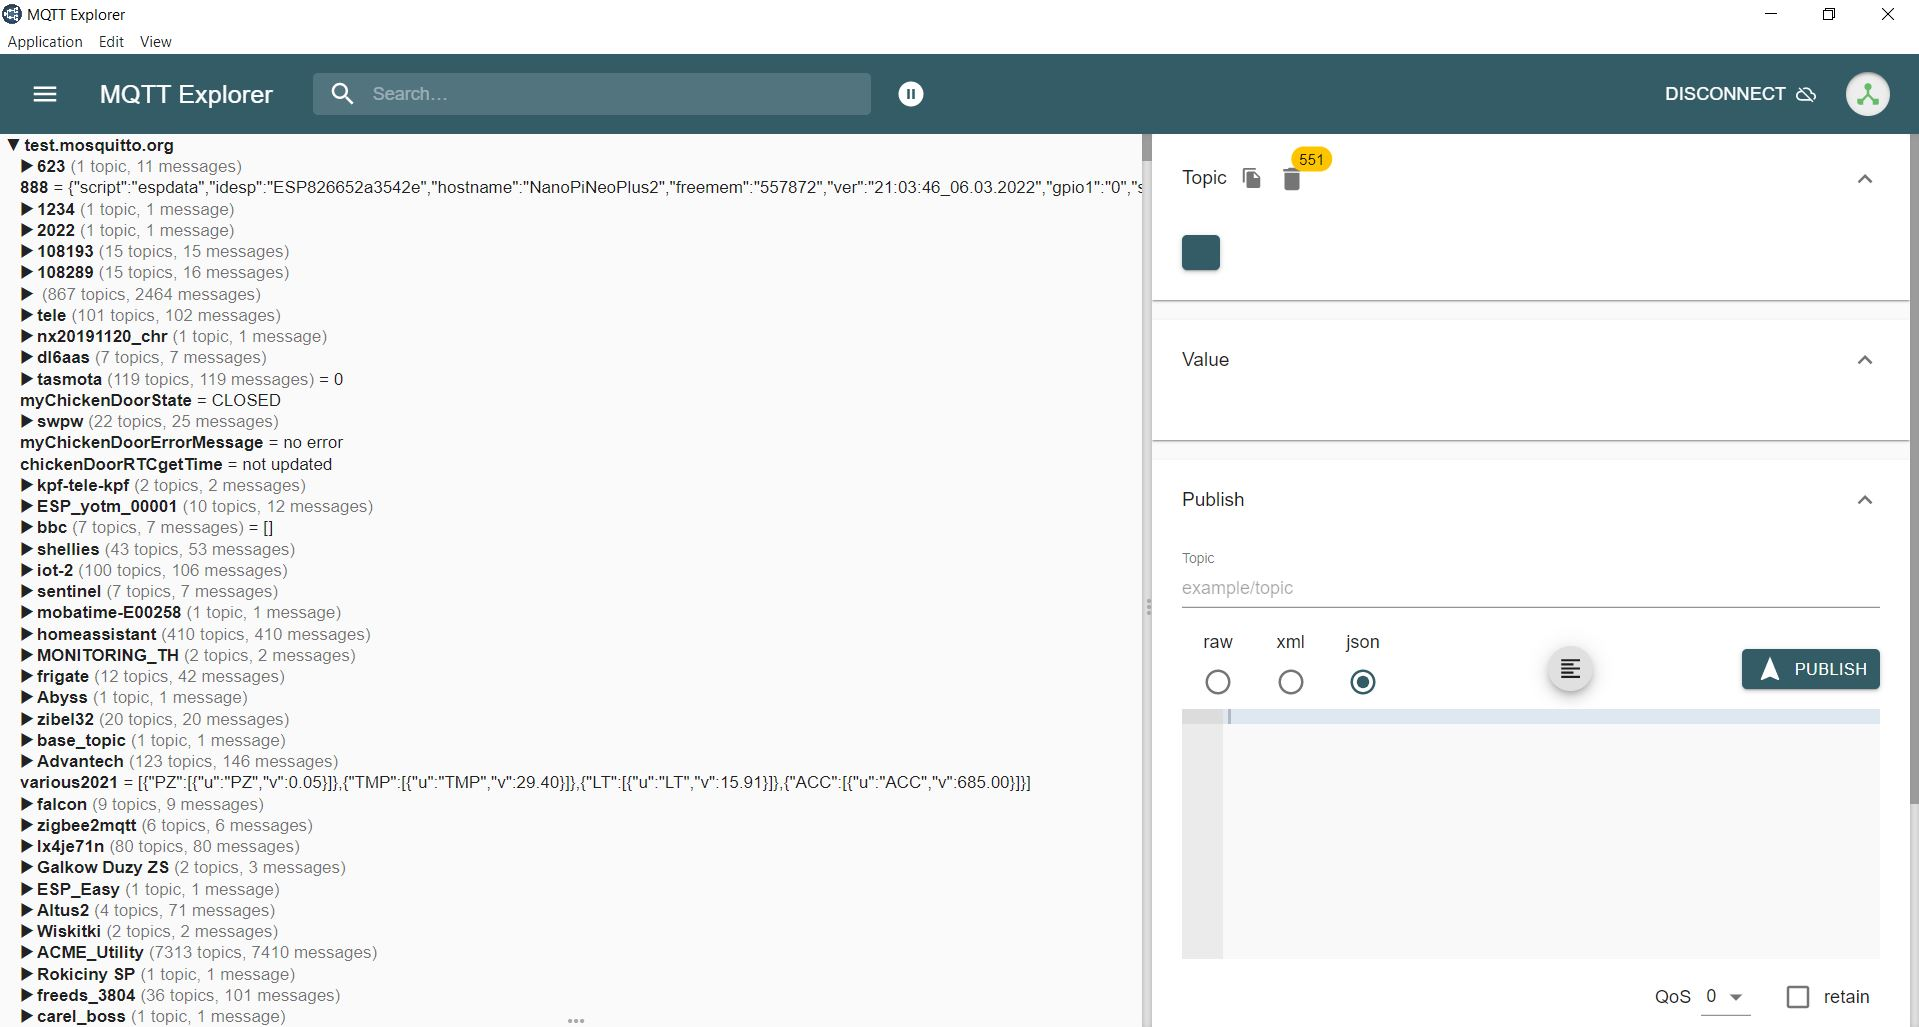
\includegraphics[width=1\textwidth]{pics/MQTTExplorerTestDemo.JPG}
    \caption{MQTT-Explorer nachdem Login}
\end{figure}








\section{.Net}
\setauthor{Sebastian Egger}


\subsection{.Net Core und .Net Framework}

In unserem Projekt verwenden wir .Net Core, eine alternative dazu wäre .NetFramework.
Beides sind Frameworks, welche für die Erstellung serverseitiger Anwendungen verwendet werden. 
.Net Core und .Net Framework haben manche funktionale Komponenten gemeinsam und können Ihren Code auch über die beiden Plattformen hinweg gemeinsam nutzen.

\subsubsection*{ Was wird unter .Net Framework und .Net Core verstanden}
Bisher wurde .NetFramework genützt um sowohl .NET Desktop-Anwendungen als auch serverbasierte Anwendungen zu erstellen.
.NET Core wiederum dient der Erstellung von Serveranwendungen, die unter Windows, Linux und Mac laufen.
Bei .NET Core handelt es sich in erster Linie um ein Open-Source-Framework mit Multiplattform-Unterstützung.


\subsubsection*{.Net Framework Vorteile}
Während .NET Core die Zukunft der Anwendungsentwicklung ist und das .NET Framework in der Zukunft ablösen wird, wird die jahrelange Verwendung von .NET Framework nicht so schnell vergehen!
Spricht man über .NET Framework vs. .NET Core im heutigen Kontext, so hat .NET Framework immer noch einige praktische .NET-Vorteile.

.Net Core benötigt derzeit für unerfahrene Programmierer einen größeren Lernaufwand als bei .Net Framework. 
Ein weiterer Vorteil gegenüber .Net Core ist die Wartung bestehender Anwendungen. 
Nachdem .Net Framework sich seit Jahren im Einsatz befindet, wurden die meisten .Net Anwendungen mittels .Net Framework geschrieben. 
Ein weiterer großer Vorteil von .Net Framework ist die Stabilität der Platform. 

Microsoft hat verkündet, dass die aktuelle Version des Microsoft .NET Framework (Version 4.8) die letzte Version sein wird und es danach kein größeres .NET Framework-Update mehr geben wird.
Das bedeutet die Entwicklung von .Net Framework schreitet nicht mehr voran, aber somit können auch keine durch Updates verursachten Bugs mehr entstehen.

\subsubsection*{.Net Core Vorteile}

Wie bereits oben erwähnt ist .Net Core ein Open-Source-Framework, welches sich kontinuierlich durch offene Beiträge verbessert.
Ein weiterer Vorteil ist die plattformübergreifende Kompatibilität, damit bei Verwendung eines Computers mit Linux oder macOS als Betriebssystem trotzdem Apps, welche unter Windows laufen, verwendet werden können.
Mit .Net Core entwickelten Apps wird Benutzern die Möglichkeit geboten, diese Apps nicht nur unter Windows zu verwenden, sondern auch auf Linux oder macOS. Diese Flexibilität entfällt bei Entwicklungen mit .Net Framework.

Es gibt natürlich noch einige weitere Vorteil von .Net Core, die hier nicht erwähnt wurden.

\subsection{Visual Studio Code}
Visual Studio Code ist ein Code Editor mit vielen Funktionen.
Wie bereits im Kapitel .Net angesprochen, gibt es sehr viele Extensions
in diesem Editor, welche zum Beispiel eine Visualisierung von Inhalten einer Sqlite Datenbank
ermöglicht oder als Latex Editor genutzt werden kann.

\subsection{Visual Studio}
Visual Studio ist ein Code Editor, welcher von Microsoft entwickelt wurde, um eine
benutzerfreundliche Programmierumgebung anzubieten. Seit 2008 wird jedes 
zweite Jahr ein neues Visual Studio mit mehr Funktionen, welche dem Benutzer 
beim Programmieren das Leben vereinfachen, veröffentlicht. 

\subsubsection*{Was ist Swagger und Verwendung von Swagger in unserem Projekt}

Swagger ist eine Sammlung von Open-Source-Werkzeugen, um HTTP-Webservices (auch HTTP API oder REST-like API) zu entwerfen, zu erstellen, 
zu dokumentieren und zu nutzen.
In diesem Projekt wurde Swagger verwendet, um die API zu beschreiben und zu testen.
Swagger bietet nicht nur die Zusammenarbeit mit C\# an sondern auch mit anderen Programmiersprachen wie zum Beispiel
JAVA, JavaScript, Groovy und noch weitere Programmiersprachen, die hier nicht explizit erwähnt werden. 

\subsubsection*{Wie wird ein Swagger in C\# eingebunden}
In C\# kann man Swagger durch ein NuggetPackage Namens Swashbuckle.AspNetCore verwenden.
Durch dieses NuggetPackage kann ein Swagger nun in eine WebApi, wie in nachfolgender Abbildung implementiert werden:


\begin{figure}[H]
    \centering
    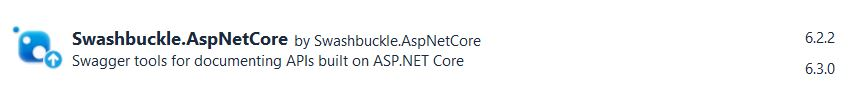
\includegraphics[width=1\textwidth]{./pics/SwaggerNuggetPackage.JPG}
    \caption{DotNet6ConApp}
\end{figure}


Die im Projekt verwendete Implementation wird im Unterkapitel Verwendung von Swagger im Projekt dargestellt.


\subsection {DotNet 5 vs DotNet 6}

Die Entwicklung der Diplomarbeit startete schon mit Sommerbeginn 2021 und .Net6 wurde erst im November 2021 released. 
Aufgrund der schon vorhandenen Kentnisse in .Net5 und der im .Net6 bei Standardkonfiguration nicht vorhandenen Methoden / Usings Unterstützung (siehe nachfolgende Abbildungen)
wurde beschlossen, währen der Umsetzung nicht die Entwicklungsumgebung zu ändern.

Eine Migration von .Net5 auf .Net6 umfasst in der Regel dann das Umstellen aller Paketversionen auf die neueste .NetVersion.
Hier sollten im Bedarfsfall dann nur wenige Änderungen notwendig werden und sollten dann auch aufgrund des längeren Supports von .Net6 
und der Vorteile rund um Performance, die bei eventueller Ausführung in der Cloud sicherlich auch positive Auswirkungen auf die 
Bedarfskosten mit sich bringen kann, in Erwägung gezogen werden.

Persönlich empfundener Nachteil bei der Lesbarkeit des Codes:

\begin{figure}[H]
    \centering
    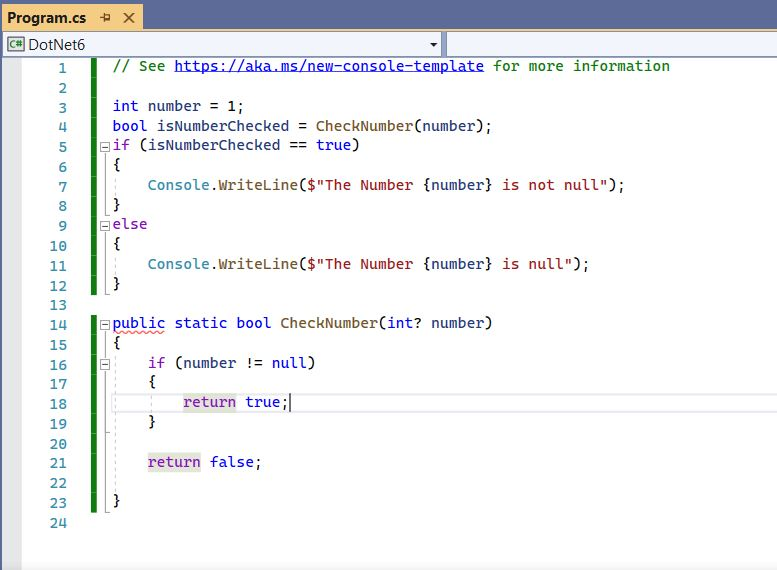
\includegraphics[width=0.7\textwidth]{./pics/DotNet6ConApp.JPG}
    \caption{DotNet6ConApp}
\end{figure}


\begin{figure}[H]
    \centering
    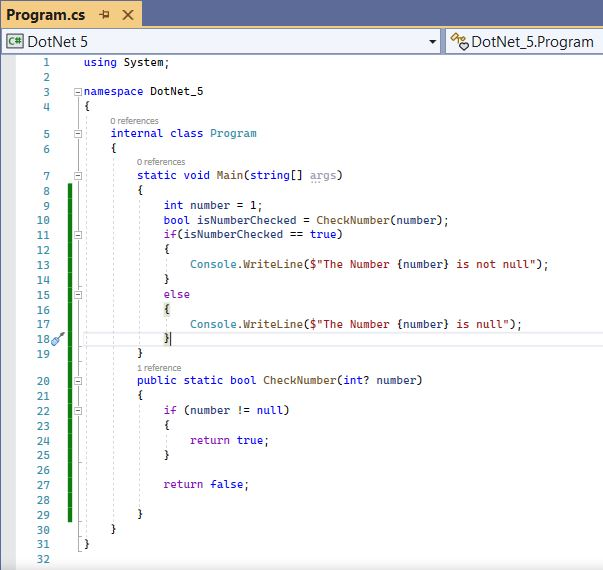
\includegraphics[width=0.7\textwidth]{./pics/DotNet5ConApp.JPG}
    \caption{DotNet5ConApp}
\end{figure}


Im Vergleich zu .Net6 ist die Unterstützung bei der Verwendung von Usings und Methoden unter .Net5 klar zu erkennen.


\subsubsection*{Was ist eine Datenbank und wofür eignet sich eine Datenbank}
Eine Datenbank ist eine Sammlung von strukturierten Informationen oder Daten, die typischerweise elektronisch in einem Computersystem gespeichert sind.
Solch eine Datenbank wird meistens von einem Datenbankverwaltungssystem abgekürzt DBMS gesteuert und sie besteht aus Tabellen, in welchen die Daten gespeichert sind.
Auf diese gespeicherten Daten kann mittels SQL-Abfragen zugegriffen werden.



\subsubsection*{Warum Sqlite und nicht SqlServer als Datenbank:}

In diesem Projekt wird eine Sqlite-Datenbank verwendet, weil die Datenbank im Vergleich zu einem Microsoft SQL Server eine kleinere
Version ist und sich sehr gut für Endgeräte eignet, da der Raspberry Pi nur über einen begrenzten Speicher verfügt.
Weiters muss auch Rücksicht auf die Architektur vom ARM genommen werden, denn die Version muss für die CPU Architektur geeignet sein.
Hinweis: Microsoft stellte erst mit SQL Server 2017 die erste Version auf Linux zur Verfügung, aber erst mit der Version 2019 sind die meisten
Funktionen wie unter Windows verfügbar.

\subsubsection*{Überprüfung einer Sqlite Datenbank}
Zum Überprüfen einer Sqlite Datenbank eignet sich in Visual Studio Code die Extension "SQLite", 
welche das Innenleben einer SQLite Datenbank veranschaulicht.

\begin{figure}[H]
    \centering
    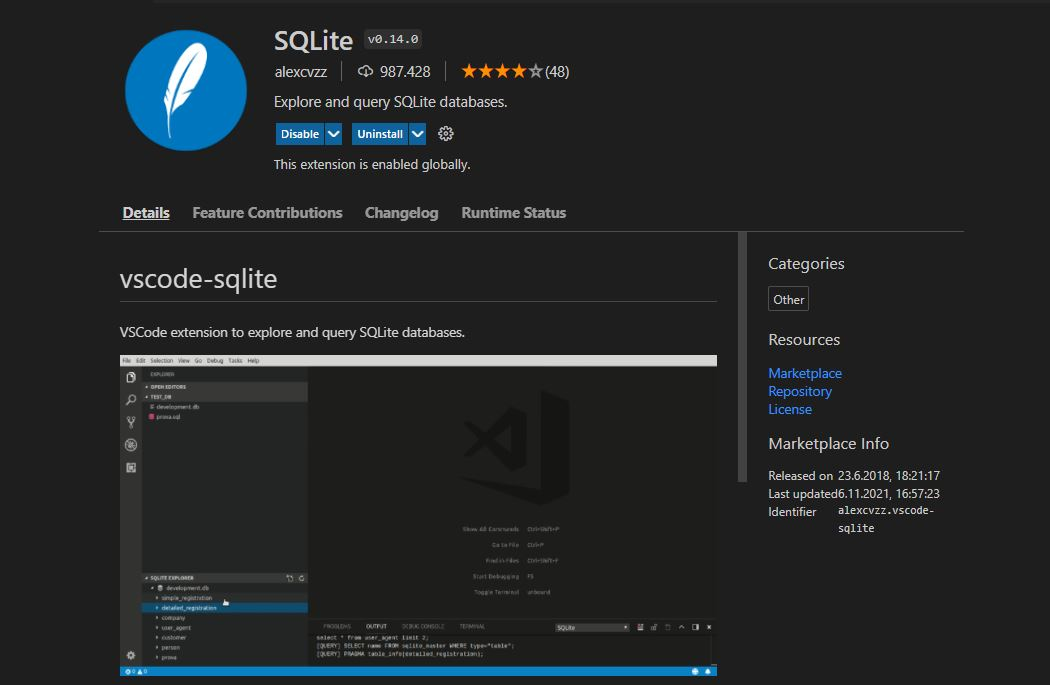
\includegraphics[width=0.8\textwidth]{./pics/SQLiteVSCodeExtension.JPG}
    \caption{SQLite Extension für Visual Studio Code}
\end{figure}

\begin{figure}[H]
    \centering
    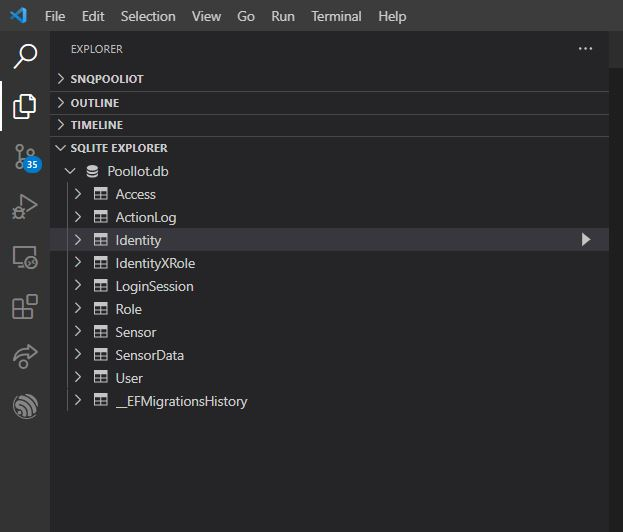
\includegraphics[width=0.8\textwidth]{./pics/SQLiteDatabaseStructure.JPG}
    \caption{Innenleben der SQLite Datenbank}
\end{figure}



\subsubsection*{Asynchrone Programmierung und Implementierung in C\#}
Es sollte wenn möglich immer asynchron programmiert werden, weil es Zeit spart, denn Prozesse können dadurch parallel ausgeführt werden.
Somit muss ein Prozess nicht mehr auf einen anderen Prozess warten.
Ein kleines Beispiel hierfür wäre ein Frühstück, denn eine Person muss eben nicht warten bis das Toastbrot fertig ist, um sich danach erst den Kaffee zu machen, dieses Tun sollte parallel möglich sein.

In C\# gibt es die Keywörter async und await. Wenn eine Methode asynchron aufgerufen werden soll, muss die Methode im Methodenkopf als Kennung async aufweisen und einen Task als return Wert festlegen.
Um diese Methode danach aufrufen zu können, muss await vor dem Methodennamen verwendet werden.


\subsubsection*{Keyword partial C\#}
In C\# gibt es das sogenannte Keyword partial, wodurch die Implementierung von einer Methode in einer Klasse der selben Klasse jedoch in einem anderen File passieren kann.
Ein Code Beispiel im Projekt wäre die SnQPoolIot.ConApp.

In den nachstehenden 2 Abbildungen wird beschrieben wie eine Implementierung von einer partial Method erfolgt.

Im ersten Foto ist zu erkennen, dass die Klasse Program.cs partial gesetzt wurde und die Methode BeforeRun() auch das Keyword partial beinhaltet.
\begin{figure}[H]
    \centering
    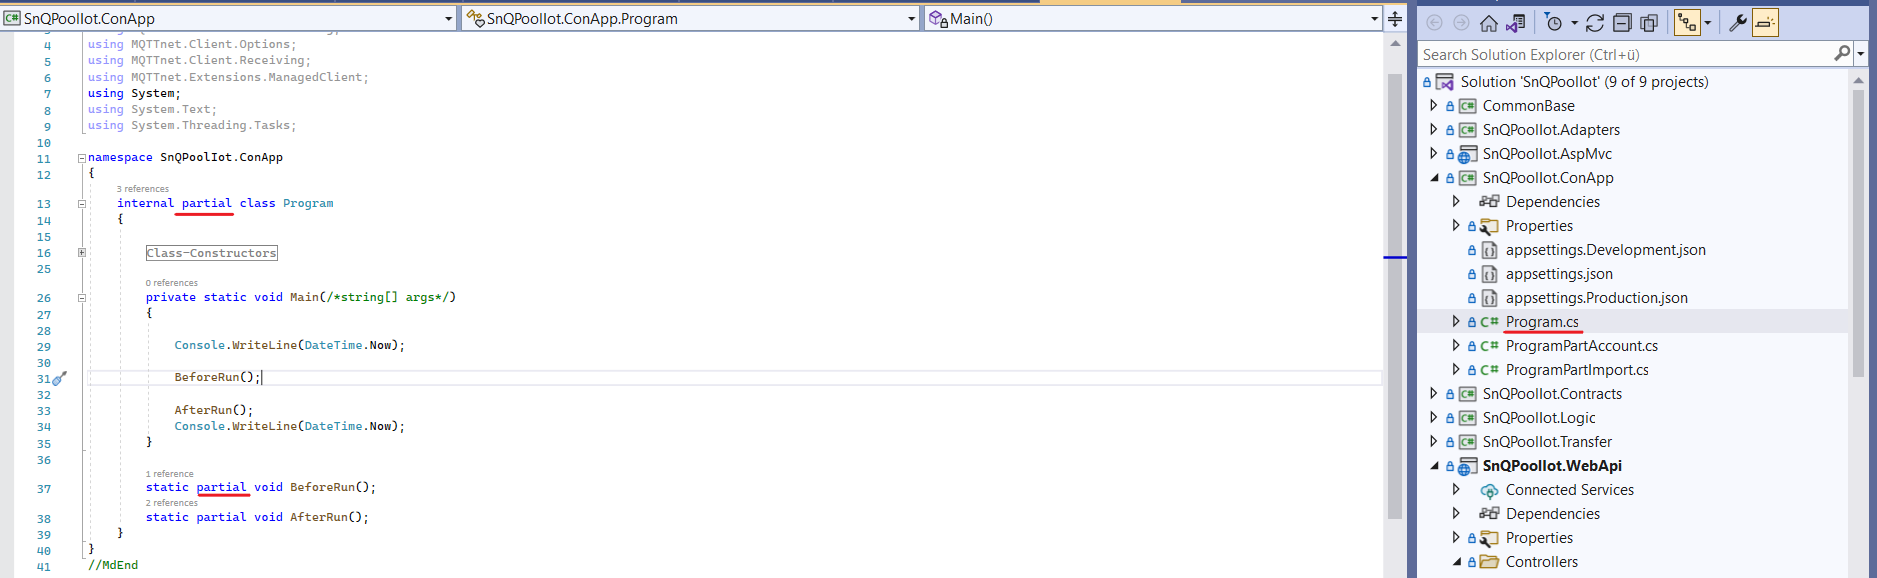
\includegraphics[width=1\textwidth]{./pics/PartialKeyword1.png}
    \caption{Implementierung partial Class und Method}
\end{figure}

Für die Implementierung in einem anderen File wird der Name des Files auf einen anderen Namen umbenannt und danach wird die Klasse wieder auf Programm.cs umgeschrieben.
Nun erkennt C\# das es sich um eine partial Class handelt und somit können nun die Methoden, welche in der Klasse partial sind, aber in einem anderen File liegen, umgeschrieben werden. 
\begin{figure}[H]
    \centering
    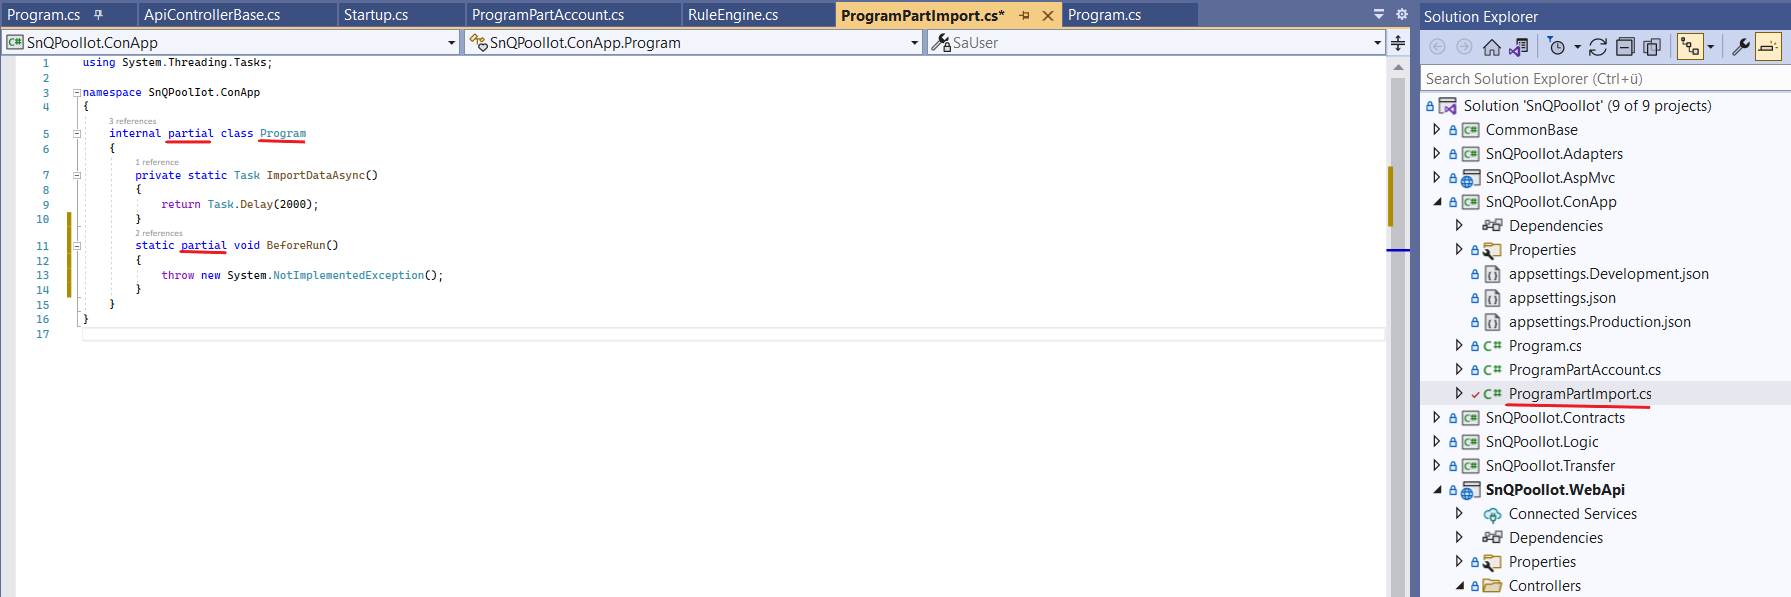
\includegraphics[width=1\textwidth]{./pics/PartialKeyword2.png}
    \caption{Implementierung partial Class und Method}
\end{figure}


\section{Telegram}
\setauthor{Sebastian Egger}
Telegram ist ein Messaging-Dienst wie WhatsApp, welcher auf Smartphones und Computer vorzufinden ist.
In diesem Projekt wird Telegram auch zum Versenden und Empfangen von Messages verwendet, jedoch über einen sogenannten Bot.
Telegram hat ein eigenes Botnetzwerk, wodurch Messages über das Internet gesendet werden können.
Um einen Bot für solche Zwecke erzeugen zu können, muss bei dem sogenannten BotFather ein Bot erzeugt werden.

\begin{figure}[H]
    \centering
    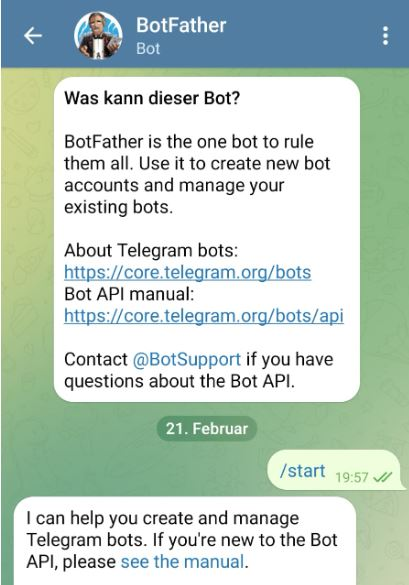
\includegraphics[width=0.8\textwidth]{./pics/BotFather.JPG}
    \caption{Erzeugen eines Bots über den BotFather}
\end{figure}

Sobald der BotFather gestartet wurde, kann über den Befehl /newbot ein neuer Bot erzeugt 
werden, indem eine Person dem Bot einen Namen und einen nicht existenten Usernamen,der mit bot endet, zuweist.
Wenn dieser Vorgang durchgeführt wurde, kann auf den Bot über HTTP Requests zugegriffen werden.

\begin{figure}[H]
    \centering
    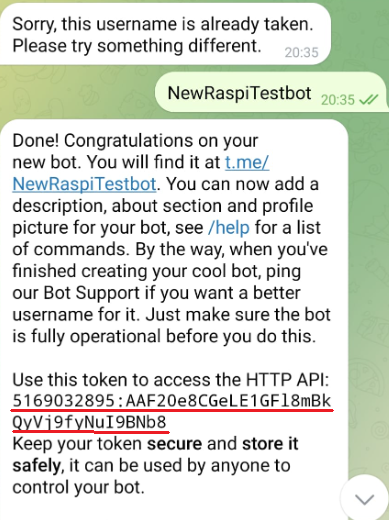
\includegraphics[width=0.8\textwidth]{./pics/TelegramBotCreatedToken.png}
    \caption{Beispiel eines Tokens der zum Zugriff auf die API benötigt wird.}
\end{figure}

Durch diesen Token kann über das Internet Messages gesendet werden oder auch die ChatId, welche
eine große Rolle im Backend des Projektes spielt, herausfinden. Der Befehl um die ChatId zu erlangen lautet:

https://api.telegram.org/bot(Token)/getMe 
\\danach kann eine Message über den Befehl \\
https://api.telegram.org/bot(Token)/sendMessage?chat\_id=(chatId)\&text=\"Text\" ddddddd 
\\gesendet werden.

\section{Begriffserklärungen}

\subsection{C\#}
C\# ist eine objektorentierte Programmiersprache, welche von Microsoft entwickelt
wurde

\subsection{ARM}
ARM stand für Acorn RISC Machines, später für Advanced RISC Machines 
und ist einer der meistverbreiteten Mikroprozessoren.


\begin{spacing}{1}
	\chapter{Projektumsetzung}\label{chapter:projectdesc}
	\end{spacing}
	



\section{Projektmanagement}
Das Projekt ist im Softwarebereich mittels Scrum und im Hardwarebereich mittels einer hybriden Projektentwicklung entwickelt worden.

\subsection{Scrum}
Scrum ist ein agiles Vorgehensmodell für Projektmanagement
und kommt zum Einsatz wenn viele Entwicklungsprojekte zu komplex sind, um sie in einen vollumfassenden Plan zu fassen.
Aus diesem Grund ist ein wesentlicher Teil der Anforderungen und Lösungen zu Beginn unklar. 
Diese werden schrittweise erarbeitet, indem Zwischenergebnisse geschaffen werden.
Durch Scrum wird die Projektlaufzeit in Etappen, so genannte Sprints, eingeteilt und
am Ende jedes Sprints soll jeweils ein funktionsfähiges Zwischenprodukt stehen.
Die Einteilung wie lange ein Sprint dauert wird intern geregelt.
In diesem Projekt war die Dauer eines Sprintes einen Monat lang.
\cite{Scrum}

\subsection{Hybride Projektentwicklung}
Hybride Projektentwicklung wird meist im Hardwarebereich verwendet.
Es ermöglicht eine schnellere Produktion von Hardwareteilen.
In diesem Projekt ist es bei dem Zusammenbau für den Raspberry verwendet
und für die Produktion einer Schwimmboje vorgesehen worden.



\subsection{Zusätzliche Vereinbarungen der Diplomarbeit}
Zusätlich zu den Projektentwicklungskonzepten wurde jede zweite Woche ein Projektbericht veröffentlicht, um die Diplomarbeitsbetreuer auf dem Laufenden zu halten.

\begin{figure}[H]
    \centering
    
\includegraphics[width=1\textwidth]{pics/AusschnittProjektberichte.png}
    \caption{Ausschnitt aus den Projektberichten}
\end{figure}


In den Projektberichten sind die fertigen Meilensteine und die  Meilensteine an denen gearbeitet wurde, mittels einer Projektampel veranschaulicht.
Eine Projektampel sagt aus, ob sich ein Projekt in Gefahr, in Verzug oder im grünen Bereich befindet.


\begin{figure}[H]
    \centering
    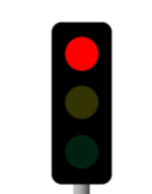
\includegraphics[width=0.7\textwidth]{pics/Projektampel.png}
    \caption{Visualisierung einer Projektampel}
\end{figure}

\section{Backend Projekt-Überblick}
\setauthor{Sebastian Egger}

Das Backend setzt sich aus 9 Projekten zusammen, welches mithilfe des von Herrn DI Professor Gerhard Gehrer zur Verfügung gestellten Frameworkes SmartNQuick entwickelt wurde.
Das Backend wurde in der Sprache C\# in .Net 5 programmiert und als Code Editor wurde
Visual Studio 2019 und 2022 verwendet.
 


\begin{figure}[H]
    \centering
    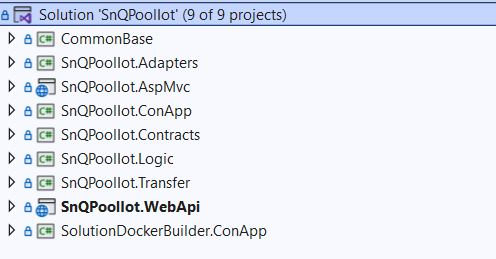
\includegraphics[width=0.7\textwidth]{pics/Projektmappe.JPG}
    \caption{Projektmappe}
\end{figure}


\begin{itemize}
    \item CommonBase
    \\
    In CommonBase befinden sich Klassen und Methoden, die wiederverwendbar sind, um Codeverdoppelung zu vermeiden.
\end{itemize}


\begin{itemize}
    \item SnQPoolIot.Adapters
    \\
    SnQPoolIot.Adapters bietet einen direkten Zugriff auf die Logic.
Der Zugriff auf die Logic kann dadurch entweder direkt erfolgen oder per Rest über die WebApi.
\end{itemize}

\begin{itemize}
    \item SnQPoolIot.WebApi
    \\
    Der Zugriff auf die Messwerte wird durch Rest-Zugriffe in SnQPoolIot.WebApi provided.
    Auf die Daten kann aber nur per Login mit einem gültigen Account zugegriffen werden.
    Genaueres zu den einzelnen HTTP-Requests ist im Kapitel HTTP und Verwendung in unserem Backend zu finden.
\end{itemize}

\begin{itemize}
    \item SnQPoolIot.Contracts
    \\
    SnQPoolIot.Contracts beinhaltet alle notwendigen Schnittstellen und Enumerationen des Projektes.
    Hier werden die Entitäten als Interfaces angelegt.
\end{itemize}


\begin{itemize}
    \item SnQPoolIot.Logic
    \\
    SnQPoolIot.Logic ist das Kernstück des Projektes. 
    Durch die Logic können alle Daten aus der Datenbank verwendet werden. 
    Die Logic verbindet sich mit einer Sqlite Datenbank. Der Zugriff und das Erzeugen der Datenbank wird mittels Entityframework.Sqlite durchgeführt.
\end{itemize}

\begin{itemize}
    \item SnQPoolIot.Transfer
    SnQPoolIot.Transfer verwaltet die Transferobjekte für den Datenaustausch zwischen den Layern.
\end{itemize}


\begin{itemize}
    \item SnQPoolIot.AspMvc
    SnQPoolIot.AspMvc ist ein Ersatz für das Frontend.
    Hier werden die Funktionen z.B.: das Einloggen eines Users oder Anzeigen von Messwerten dargestellt.
\end{itemize}

\begin{itemize}
    \item SnQPoolIot.ConApp
    In SnQPoolIot.ConApp werden User mit verschiedenen Rechten angelegt, die für die Authentifizierung benötigt werden.
\end{itemize}



\subsection{SnQPoolIot.Logic}
Wie  bereits im Backend Projekt-Überblick beschrieben, befindet sich in SnQPoolIot.Logic die Datenbank mit den Zugriffen.
Die Datenbank wird mithilfe des NuggetPackage Microsoft.Entityframework.Sqlite, den Befehlen:
dotnet ef migrations add InitDb und dotnet ef database update, welche in der Developer-PowerShell 
im Visual Studio ausgeführt werden müssen um Migrations zu erzugen und um die Datenbank mit den erzeugten Migrations upzudaten, 
und einem DBContext, welcher die Configuration der Datenbank mit sich bringt, automatisch erstellt. 

\begin{figure}[H]
    \centering
    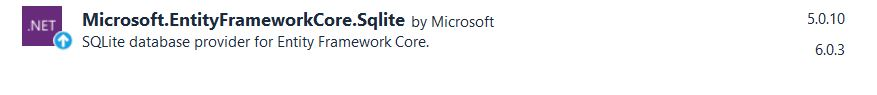
\includegraphics[width=1\textwidth]{pics/EntityFrameworkSqlLiteNuggetPackage.JPG}
    \caption{NuggetPackage für Entityframework mit Sqlite}
\end{figure}


\begin{figure}[H]
    \centering
    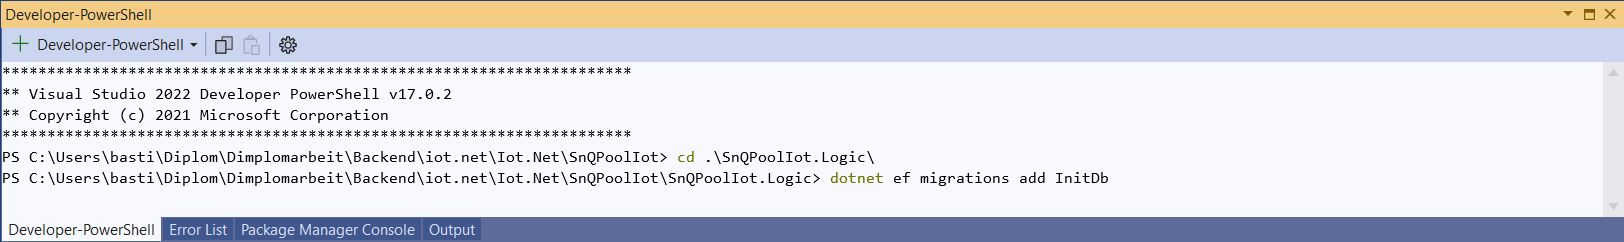
\includegraphics[width=1\textwidth]{pics/DeveloperPowerShellMigration.JPG}
    \caption{Befehl zum Erzeugen von Migationen}
\end{figure}

\begin{figure}[H]
    \centering
    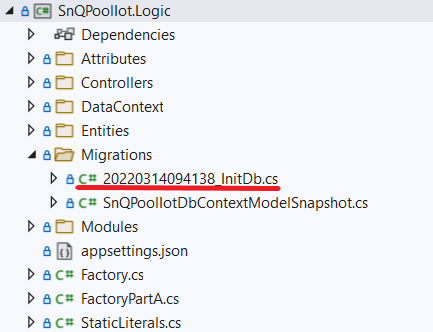
\includegraphics[width=1\textwidth]{pics/MigrationCreated.png}
    \caption{Erzeugte Migrationen in der Logik}
\end{figure}

\begin{figure}[H]
    \centering
    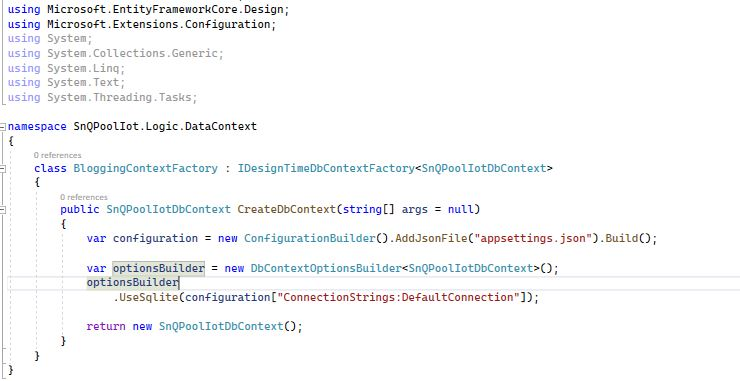
\includegraphics[width=1\textwidth]{pics/DBContext.JPG}
    \caption{DBContext zum Erzeugen einer Datenbank}
\end{figure}

Nun zu den Datenbank Zugriffen. Um auf die Messwerte zugreifen zu können, muss sich ein User zuerst authentifizieren.
Damit sich eine User authentifizieren kann benötigt er einen Account mit E-Mail und Passwort, welche in der Datenbank gespeichert sind.
Für die Authentifizierung werden die nachstehenden Tabellen benötigt:

\begin{itemize}
    \item Identity\\
    In dieser Tabelle befinden sich alle User-Accounts mit E-Mail und zugehörigem gehashtem Passwort.

    \begin{figure}[H]
        \centering
        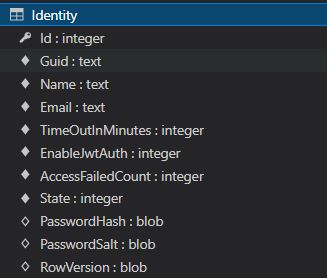
\includegraphics[width=0.7\textwidth]{pics/IdentityTableStructur.JPG}
        \caption{Identity Tabelle mit den dazugehörigen Tabellenspalten}
    \end{figure}

\end{itemize}


\begin{itemize}
    \item Role\\
    In dieser Tabelle sind alle Rollen, die es gibt, vorzufinden.

    \begin{figure}[H]
        \centering
        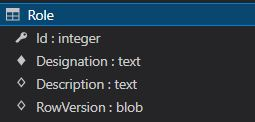
\includegraphics[width=1\textwidth]{pics/RoleTableStructure.JPG}
        \caption{Role Tabelle mit den dazugehörigen Tabellenspalten}
    \end{figure}

\end{itemize}

\begin{itemize}
    \item IdentityXRole\\
    Diese Tabelle weist einem Benutzer eine Rolle zu.
    \begin{figure}[H]
        \centering
        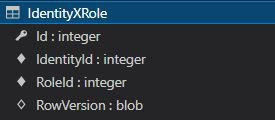
\includegraphics[width=1\textwidth]{pics/IdentityXRoleStructure.JPG}
        \caption{IdentityXRole Tabelle mit den dazugehörigen Tabellenspalten}
    \end{figure}
\end{itemize}


\begin{itemize}
    \item LogginSession\\
    Diese Tabelle zeigt alle Logins mit dem dazugehörigen User und dem SessionToken, mit dem sich der User eingeloggt hat, an.
    \begin{figure}[H]
        \centering
        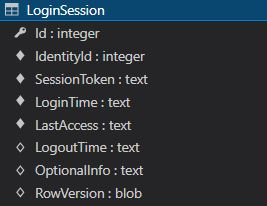
\includegraphics[width=1\textwidth]{pics/LoginSessionStructure.JPG}
        \caption{LogginSession Tabelle mit den dazugehörigen Tabellenspalten}
    \end{figure}
\end{itemize}

Sobald sich ein User authentifiziert hat, wurde zugleich eine neue Session erstellt. Nur bei ausreichender Berechtigung des authentifizierten Benutzers kann dieser sich nun die Messwerte ansehen.
Die nachstehenden Tabellen dienen zum Erfassen der Messwerte:

\begin{itemize}
    \item Sensor\\
    Diese Tabelle beinhaltet den Namen eines Sensors.
    \begin{figure}[H]
        \centering
        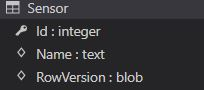
\includegraphics[width=1\textwidth]{pics/SensorTableStructure.JPG}
        \caption{Sensor Tabelle mit den dazugehörigen Tabellenspalten}
    \end{figure}
\end{itemize}

\begin{itemize}
    \item SensorData\\
    Diese Tabelle beinhaltet die Messwerte aller Sensoren und jeder Messwert ist einem Sensor zugeordnet.
    \begin{figure}[H]
        \centering
        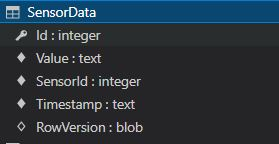
\includegraphics[width=1\textwidth]{pics/SensorDataTableStructure.JPG}
        \caption{SensorData Tabelle mit den dazugehörigen Tabellenspalten}
    \end{figure}
\end{itemize}


\subsubsection{Logging in unserem Projekt}
Um Fehlermeldungen oder Warnungen im Projekt zu speichern, wurde eine Klasse mit dem Namen LogWriter programmiert.
Diese Meldeungen werden in einer .txt gespeichert und können jederzeit gelesen werden.
\\Im nachstehenden Code ist die LogWriter Klasse zu sehen:
\\
\begin{lstlisting}[caption={Logwriter Klasse}]
using System;
using System.Collections.Generic;
using System.IO;
using System.Linq;
using System.Reflection;
using System.Text;
using System.Threading.Tasks;

namespace SnQPoolIot.Logic.Entities.Business.Logging
{
    public class LogWriter
    {
        private string m_exePath = string.Empty;
        private static LogWriter _instance = null;

        public static LogWriter Instance
        {
            get
            {
                if(_instance == null)
                {
                    _instance = new LogWriter();
                }
                return _instance;
            }
        }

        private LogWriter()
        {

        }
        public void LogWrite(string logMessage)
        {
            m_exePath = Path.GetDirectoryName(Assembly.GetExecutingAssembly().Location);
            try
            {
                using StreamWriter w = File.AppendText(m_exePath + "\\" + "log.txt");
                Log(logMessage, w);
            }
            catch (Exception)
            {
            }
        }
        public static void Log(string logMessage, TextWriter txtWriter)
        {
            try
            {
                txtWriter.Write("\r\nLog Entry : ");
                txtWriter.WriteLine("{0} {1}", DateTime.Now.ToLongTimeString(),
                    DateTime.Now.ToLongDateString());
                txtWriter.WriteLine("  :{0}", logMessage);
                txtWriter.WriteLine("-------------------------------");
            }
            catch (Exception )
            {
            }
        }
    }
}
\end{lstlisting}

Der Methode LogWrite wird durch einen Übergabeparameter die auszugebende Fehlermeldungen übergeben. Nach Ermittlung der Datei wird durch Aufruf der Methode Log 
die Fehlermeldung inklusive Zeitstempel in der Datei gespeichert.
\\
\\

\subsection{SnQPoolIot.WebApi}

\subsubsection*{HTTP und Verwendung im Backend}

HTTP ausgeschrieben Hypertext Transfer Protocoll wird zum Laden von Webseiten im Projekt verwendet.
Die verwendeten HTTP-Requests und das dazugehörige Routing ist im Projekt SnQPoolIot.WebApi implementiert.

Im Folgenden ist ein Ausschnitt des Aufbaus der WebApi dargestellt:

\begin{figure}[H]
    \centering
    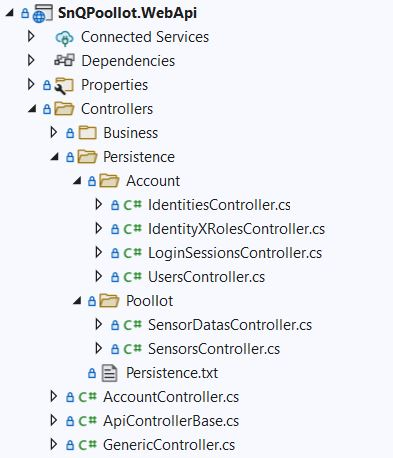
\includegraphics[width=1\textwidth]{pics/HTTPRequestsWebApi.JPG}
    \caption{Aufbau der WebApi}
\end{figure}


Das Routing der Websiten wird über die Controller gehandelt. 
Der meist genützte Controller in diesem Projekt ist der GenericController, denn er bietet allen abgeleiteten Controllern seine bereitgestellten Funktionen zur Verwendung an. \cite{Generics}

\begin{figure}[H]
    \centering
    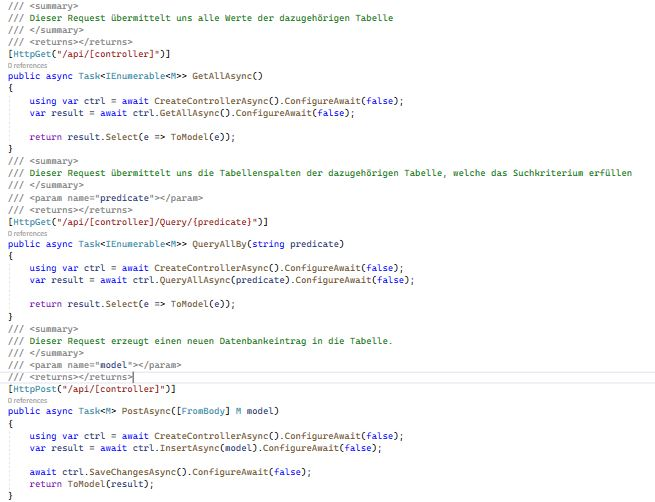
\includegraphics[width=1\textwidth]{pics/GenericControllerWebApi.JPG}
    \caption{Auszug GenericController der WebApi}
\end{figure}

Wie am Beispiel des Codeauszuges zu sehen, beinhaltet der Generic Controller einige Methoden.
\\Für die Ermittlung der Daten wird zum Beispiel eine Get-Methode \""GetAllAsync\""  eingesetzt.
\\Die Codezeile [HttpGet(\""/api/[controller]\"")] drückt aus, dass es sich bei dieser Methode um eine Get-Methode handelt 
und veranschaulicht auch das Routing der WebApi.
\\All jene Methoden, die im GenericController definiert sind, stehen demnach allen von ihm abgeleiteten Controllern zur Verfügung und können direkt verwendet werden.

Im nachstehenden Beispiel wird eine Ableitung vom GenericController dargestellt.

\begin{figure}[H]
    \centering
    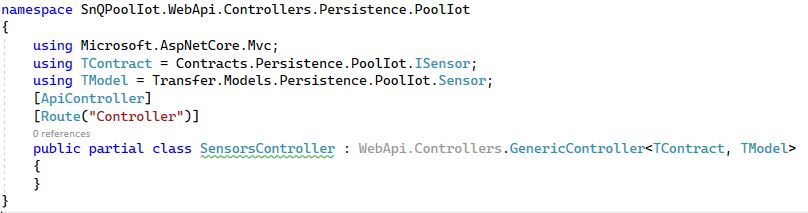
\includegraphics[width=0.7\textwidth]{pics/VerwendungGenereicController.JPG}
    \caption{Anwendung des GenericControllers der WebApi}
\end{figure}


\subsubsection*{Verwendung von Swagger im Projekt}
Zum Allgemeinen Überblick aller HTTP-Requests wird Swagger verwendet.

\begin{figure}[H]
    \centering
    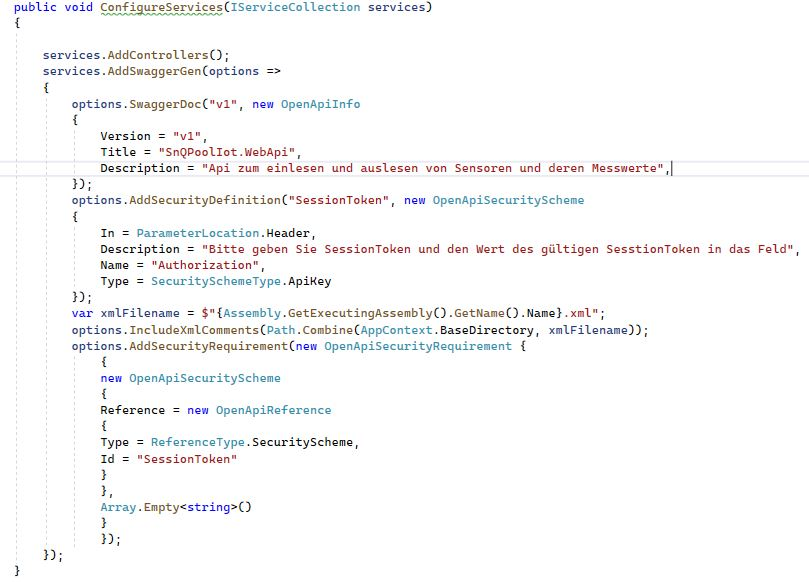
\includegraphics[width=0.8\textwidth]{pics/SwaggerImplementation.JPG}
    \caption{Implementierung von Swagger in der WebApi}
\end{figure}

In den nachstehenden Zeilen findet sich eine kurze Ablaufbeschreibung des Codes:
Sobald die Methode ConfigureServices aufgerufen wird, wird dem Service ein neuer Controller angelegt und die benötigte Konfiguration des Swaggers mit übergeben. 

Das options.SwaggerDoc gibt eine kurze Beschreibung über die WebApi an.
Im darauf folgenden Schritt wird die Authentifizierung im Projekt mittels Swagger durchgeführt. Dadurch wird gewährleistet, dass nur eingeloggte Benutzer die Möglichkeit haben Zugriffe auf HTTP-Requests durchzuführen.
Sobald die Methode fertig ausgeführt wurde startet im Browser eine Website mit allen HTTP-Requests die im Projekt implementiert sind.

\subsubsection*{Unterstützte HTTP-Requests des Projektes}
Mit Hilfe von Swagger wurden die in den nachstehenden Grafiken ersichtlichen HTTP-Requests des Backends dokumentiert:

\begin{figure}[H]
    \flushleft
    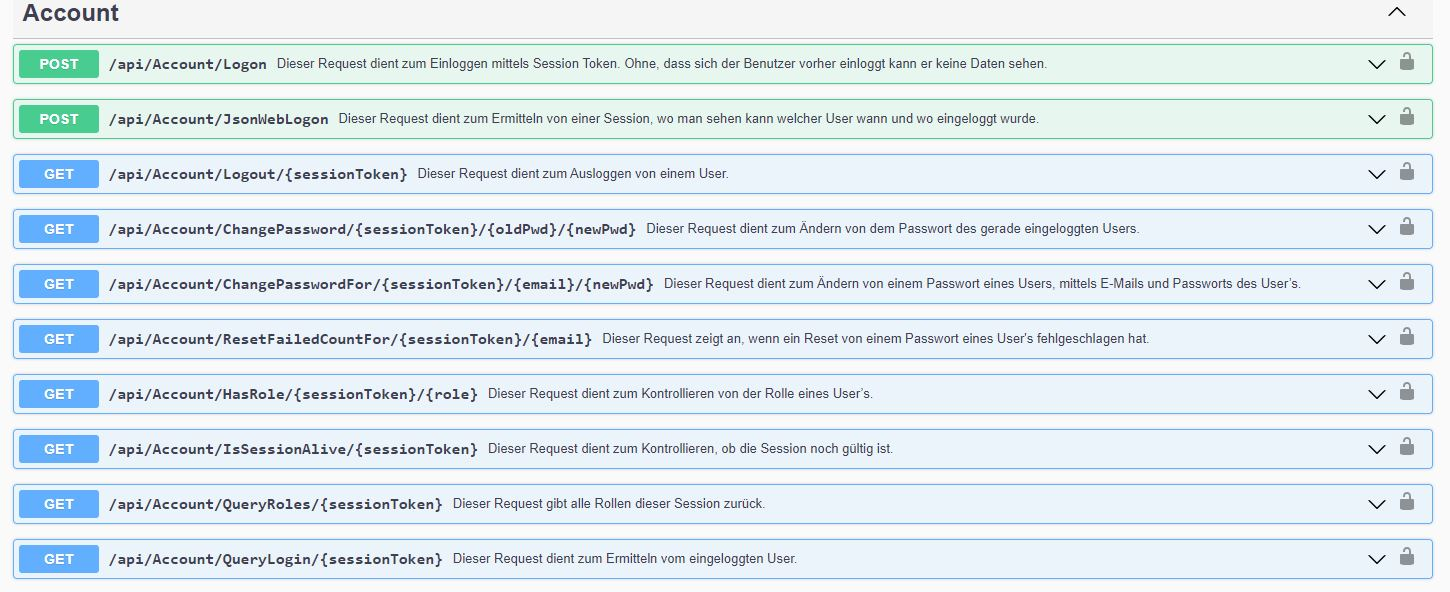
\includegraphics[width=1.6\textwidth]{pics/WebApiRequests1.JPG}
    \caption{HTTP-Requests des Projektes}
\end{figure}

\begin{figure}[H]
    \centering
    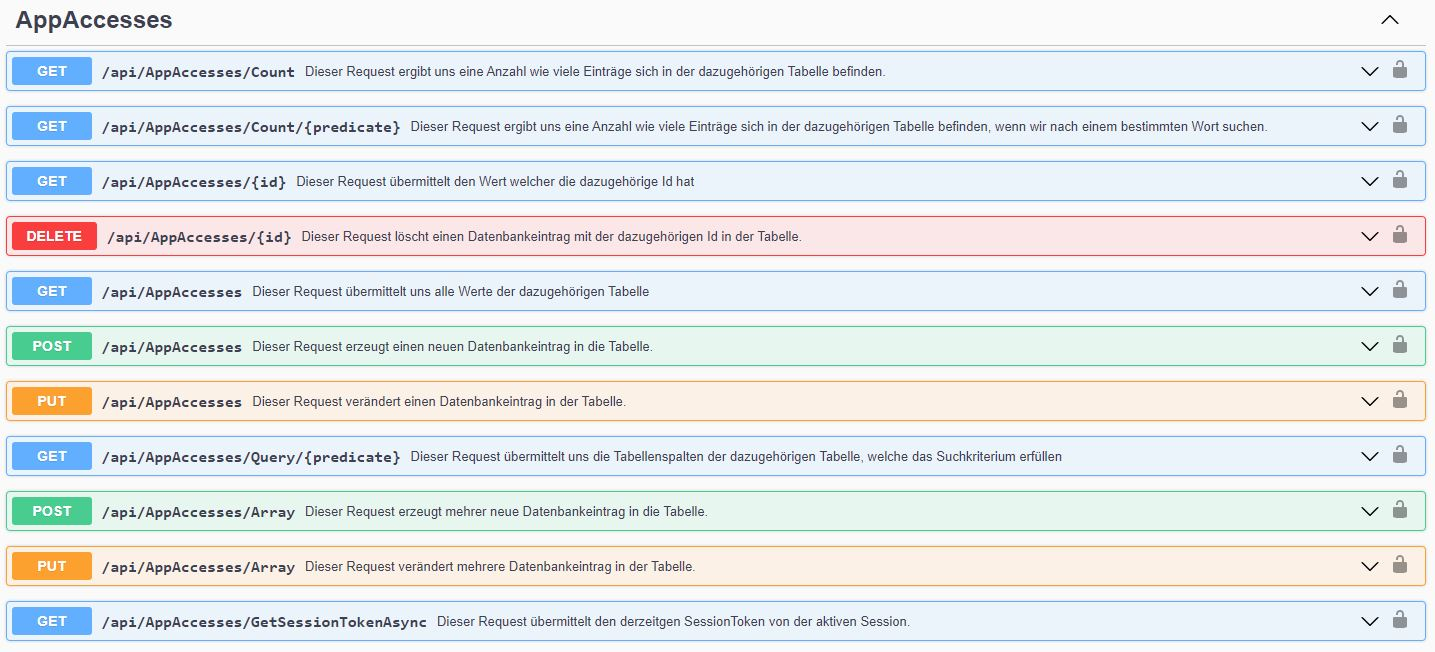
\includegraphics[width=1.6\textwidth]{pics/WebApiRequests2.JPG}
    \caption{HTTP-Requests des Projektes}
\end{figure}

\begin{figure}[H]
    \centering
    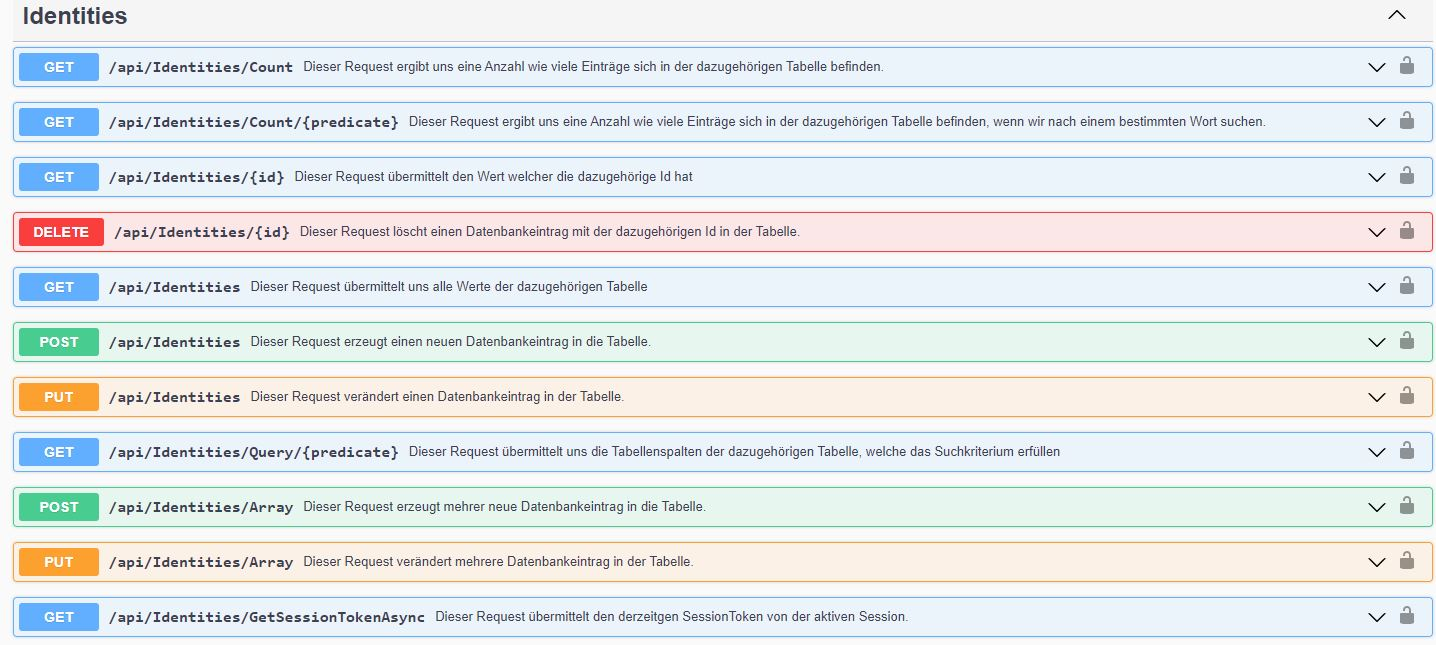
\includegraphics[width=1.6\textwidth]{pics/WebApiRequests3.JPG}
    \caption{HTTP-Requests des Projektes}
\end{figure}

\begin{figure}[H]
    \centering
    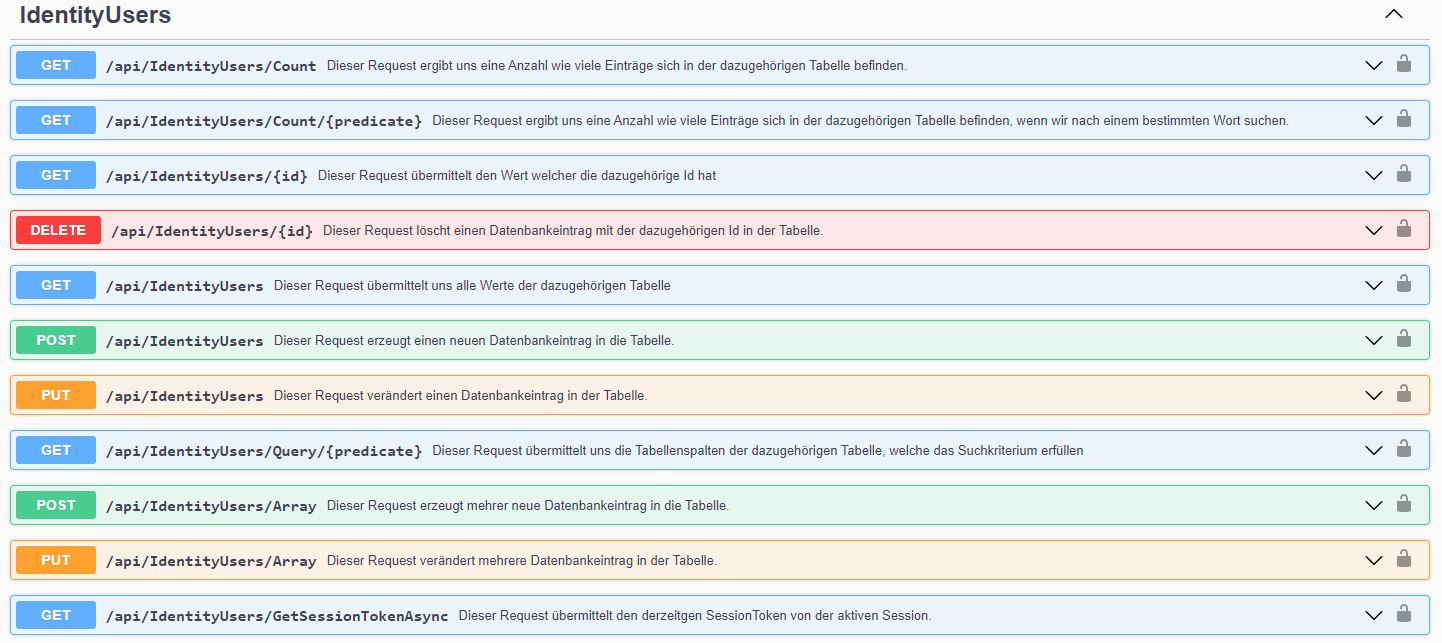
\includegraphics[width=1.6\textwidth]{pics/WebApiRequests4.JPG}
    \caption{HTTP-Requests des Projektes}
\end{figure}

\begin{figure}[H]
    \centering
    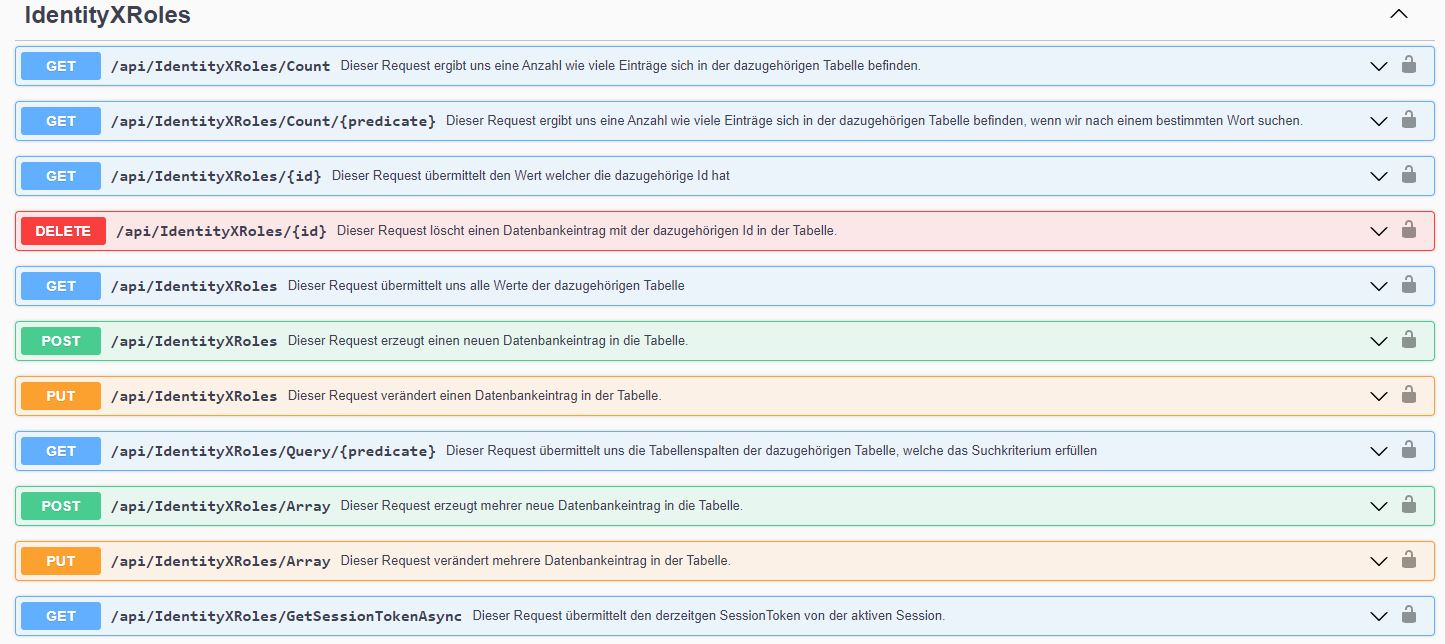
\includegraphics[width=1.6\textwidth]{pics/WebApiRequests5.JPG}
    \caption{HTTP-Requests des Projektes}
\end{figure}

\begin{figure}[H]
    \centering
    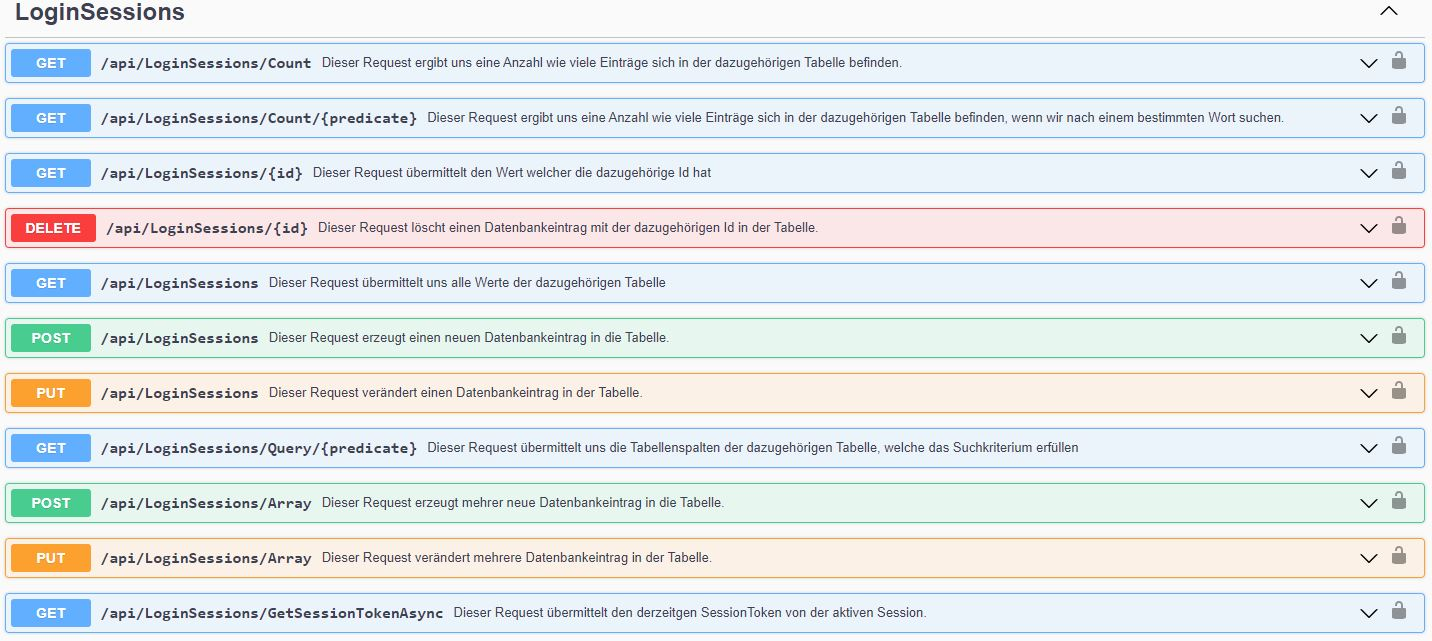
\includegraphics[width=1.6\textwidth]{pics/WebApiRequests6.JPG}
    \caption{HTTP-Requests des Projektes}
\end{figure}

\begin{figure}[H]
    \centering
    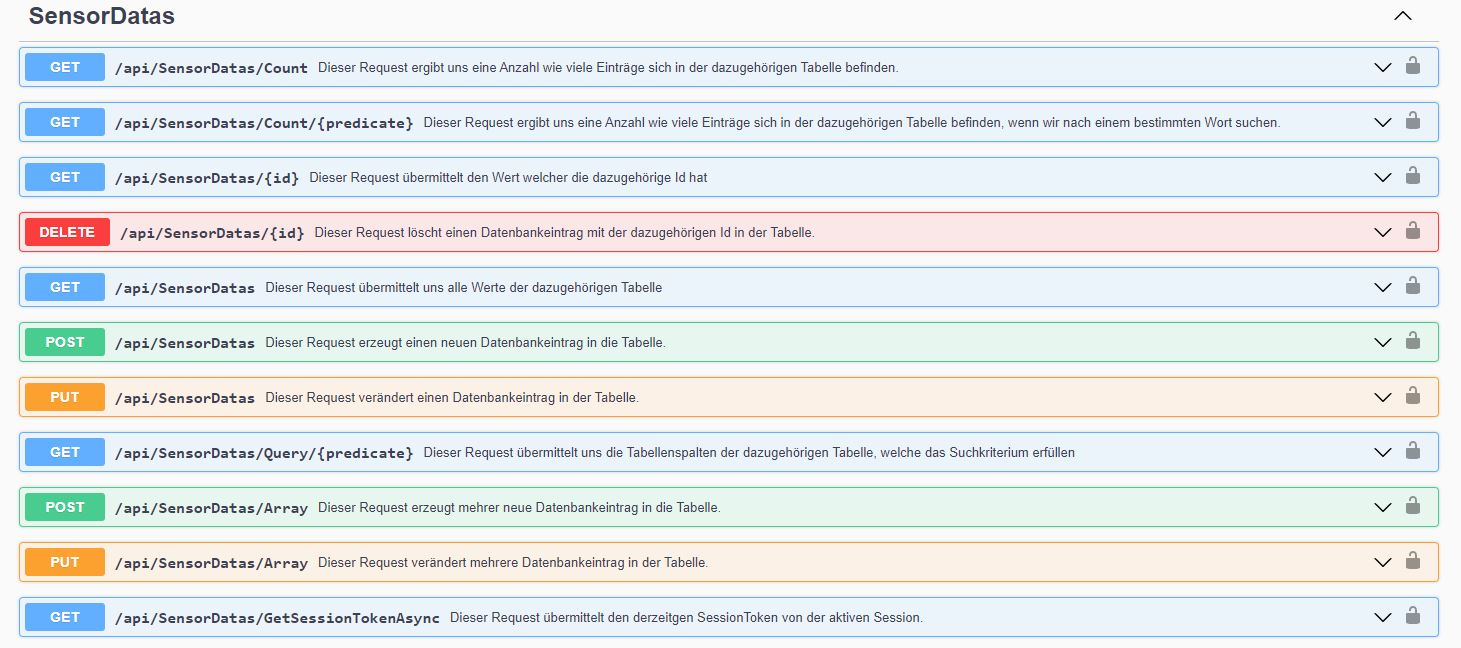
\includegraphics[width=1.6\textwidth]{pics/WebApiRequests7.JPG}
    \caption{HTTP-Requests des Projektes}
\end{figure}

\begin{figure}[H]
    \centering
    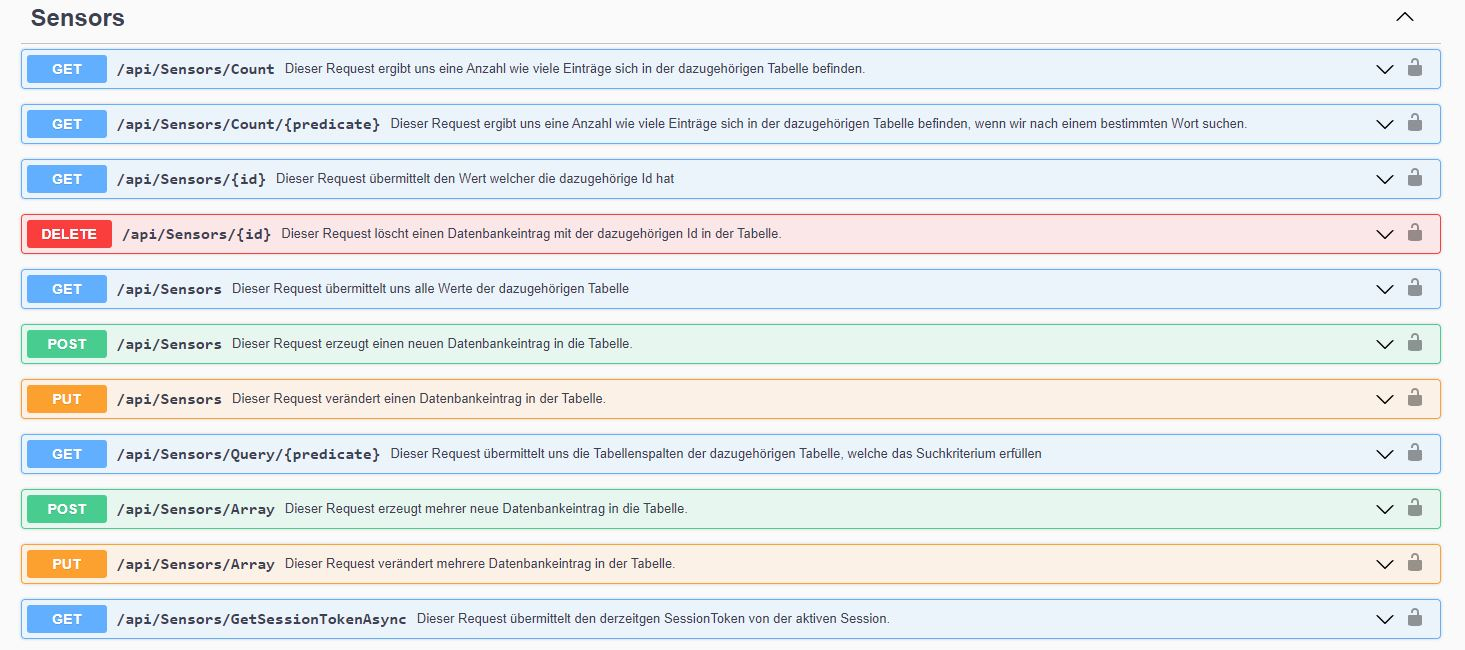
\includegraphics[width=1.6\textwidth]{pics/WebApiRequests8.JPG}
    \caption{HTTP-Requests des Projektes}
\end{figure}

\begin{figure}[H]
    \centering
    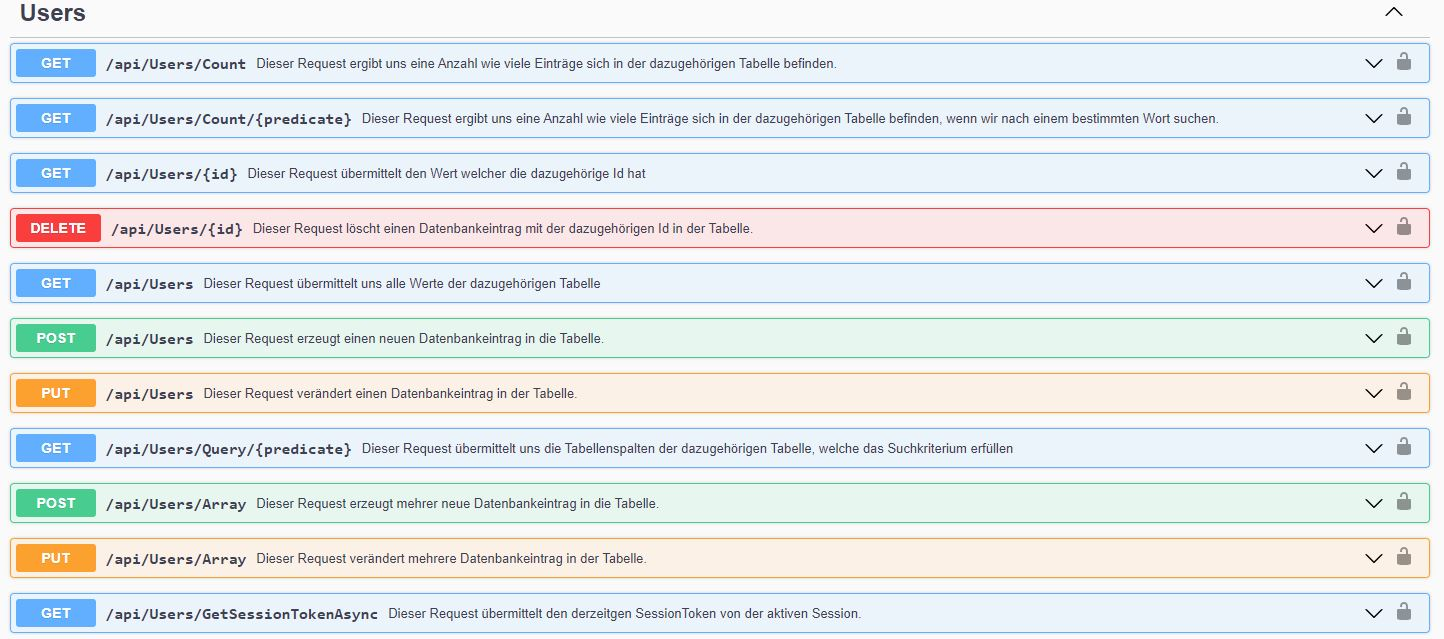
\includegraphics[width=1.6\textwidth]{pics/WebApiRequests9.JPG}
    \caption{HTTP-Requests des Projektes}
\end{figure}

\subsubsection{Implementierung von MQTT in unserem Projekt}
Das Einlesen und Überprüfen von den Messwerten soll stattfinden, sobald die WebApi läuft.
Aus diesem Grund wird die RuleEngine, 
welche den Aufruf für das Einlesen und Überprüfen der Messwerte beinhaltet, instanziert, welche gleichzeitig wie die WebApi startet.

\begin{figure}[H]
    \centering
    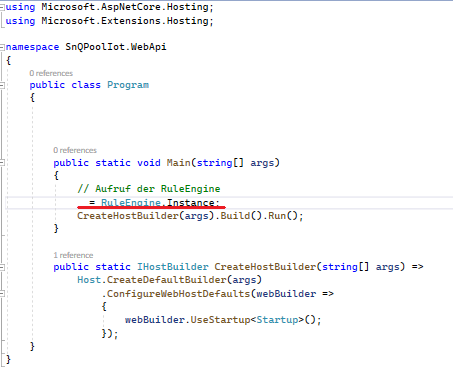
\includegraphics[width=0.6\textwidth]{pics/RuleEngineCall.png}
    \caption{Aufruf der RuleEngine}
\end{figure}

\begin{figure}[H]
    \centering
    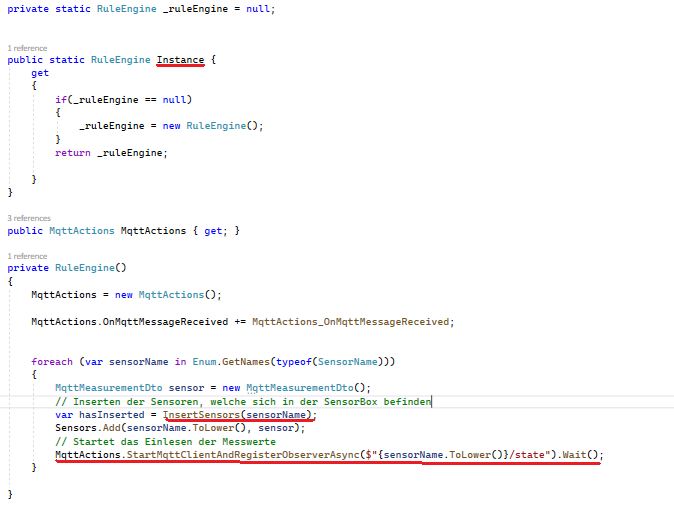
\includegraphics[width=0.9\textwidth]{pics/InstanzierenDerRuleEngineUndAufrufenDerMQTTMesswerte.png}
    \caption{Instanzieren der RuleEngine und der Sensoren zum Einlesen der Messwerte}
\end{figure}

Die einelnen Sensoren, welche in der obigen Abbildung in die Datenbank gespeichert werden,
befinden sich in dem nachstehenden enum:

\begin{figure}[H]
    \centering
    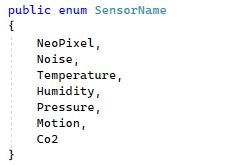
\includegraphics[width=0.9\textwidth]{pics/SensorEnum.JPG}
    \caption{Liste der Sensoren gespeichert in einem Enum}
\end{figure}

Auf diese Sensoren wird nun die Methode StartMqttClientAndRegisterObserverAsync angewendet,
welche in den nachstehenden Abbildungen und Texten beschrieben wird:

Damit das Backend einen Wert von einem Topic bekommen kann, muss auf dieses Topic scubscribed werden.
In C\# gibt es eigene NuggetPackages zum Subscriben. \\
Nachdem die NuggetPackages installiert worden sind,
kann nun ein MQTT Client mittels einer MQTTFactory erzeugt werden. Damit der MQTT Client auf den richtigen
Broker subscriben kann, muss er sogenannte MQTTClientOpions, mittels eines MQTTClientOpionsBuilder, auf sich zugewiesen bekommen.
\\Zu diesen MQTTClientOpions zählt die ClientId, die Adresse, der Username und das Passwort des Brokers, sowie
der Port auf dem der Broker läuft.
\begin{figure}[H]
    \centering
    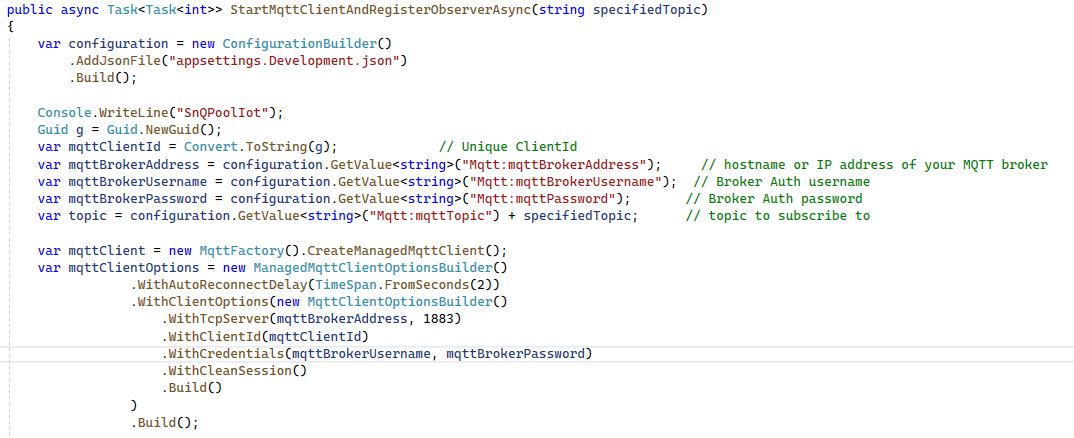
\includegraphics[width=1.3\textwidth]{pics/StartMqttClientConnections.JPG}  
    \caption{MQTT Client Konfiguration}
\end{figure}
Sobald die Konfiguration eingetragen wurde, wird dem MQTT Client nun mitgeteilt, was zu tun ist, 
wenn sich der MQTT Client connected, disconnected oder eine Nachricht bekommt.

\begin{figure}[H]
    \centering
    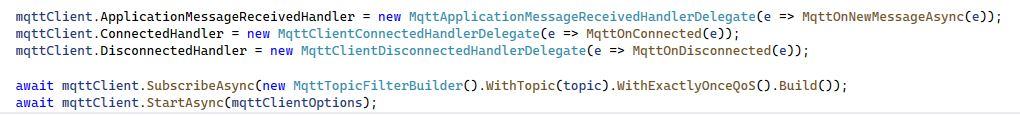
\includegraphics[width=1.3\textwidth]{pics/StartMqttClientCallMethods.JPG}  
    \caption{MQTT Cient HandlerDelegate, Subscriben und Starten}
\end{figure}

Wenn sich ein MQTT Client connected oder disconnected, wird dies 
,durch die selbstgeschrieben Logging Klasse, mitgeloggt.

\begin{figure}[H]
    \centering
    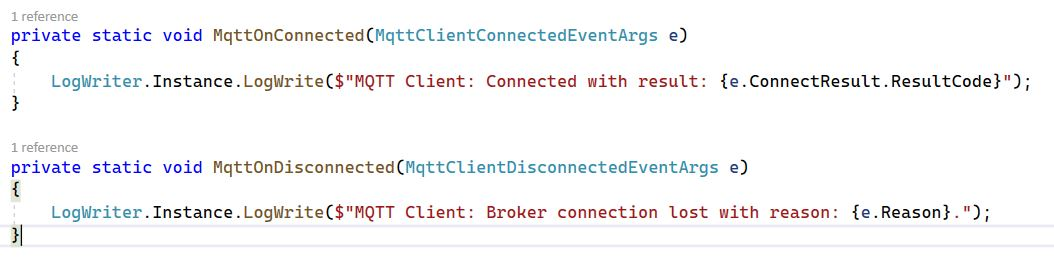
\includegraphics[width=1.1\textwidth]{pics/StartMqttClientConnectAndDisconnect.JPG}  
    \caption{MQTT Cient HandlerDelegate, Subscriben und Starten}
\end{figure}

Auch beim Empfangen einer neuen Message wird dies durch die Logging Klasse mitgeloggt,
 jedoch ist dies nicht die Hauptfunktion der Methode MqttOneNewMessage, sondern 
 das Speichern (Inserten) von Messwerten in die Datenbank.

 \begin{figure}[H]
    \centering
    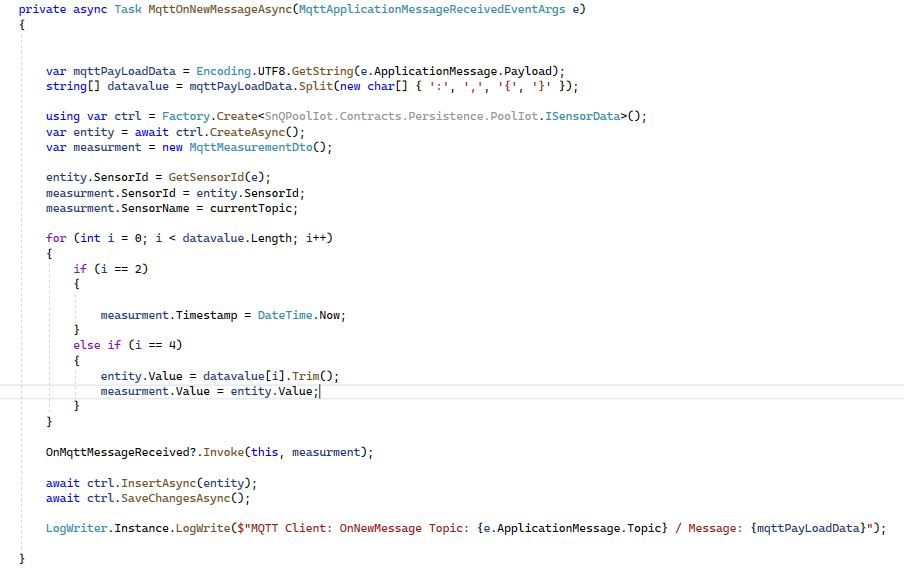
\includegraphics[width=1.1\textwidth]{pics/StartMqttClientMqttOnNewMessageAsync.JPG}  
    \caption{MQTT Cient beim Empfangen eines neuen Messwertes}
\end{figure}

Sobald ein Messwert in der Datenbank hinzugefügt wurde, wird die RuleEngine alarmiert,
welche wiederum eine Überprüfung des Messwertes durchführt. Ein gutes Beispiel hierfür ist die
Methode CheckNoiceSensorData, welche überprüft, ob der gemessene Wert über 300 db hat.

\begin{figure}[H]
    \centering
    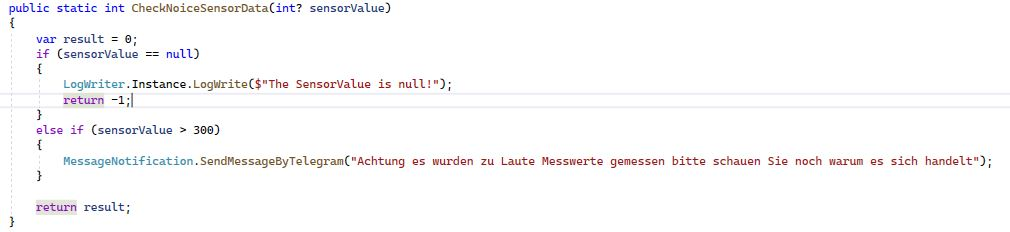
\includegraphics[width=1.1\textwidth]{pics/CheckNoiceData.JPG}  
    \caption{Kontrollieren eines Messwertes von dem Noicesensor}
\end{figure}

Sobald die Methode CheckNoiceSensorData ausgeführt wurde und der gemessene Wert über 300 db liegt,
wird der Benutzer über Telegram verständigt. Aus diesem Grund wurde die Klasse MessageNotification, 
welche die Methode SendMessageByTelegram beinhaltet, geschrieben. Wie der Name SendMessageByTelegram
schon sagt, wird in dieser Methode eine Message mittels Telegram über einen Bot versendet.
Für diesen Vorgang wird der Token, welcher für den Zugriff der HTTP API zuständig ist, und die ChatId benötigt.
Diese sind in einem appsettings.json File gespeichert und werden über die Variable configuration eingelesen.

\begin{figure}[H]
    \centering
    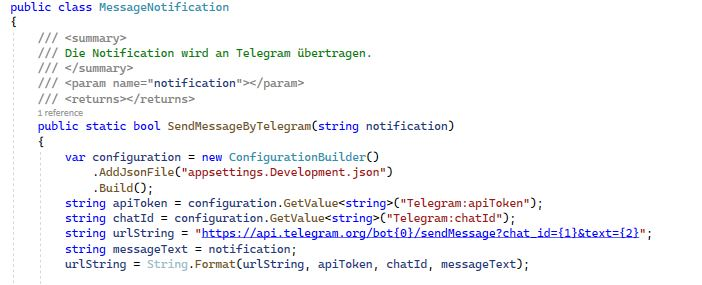
\includegraphics[width=1.1\textwidth]{pics/MessageTelegramConfiguration.JPG}  
    \caption{Configuration Daten für das Senden der Benachrichtigung}
\end{figure}

\begin{figure}[H]
    \centering
    \includegraphics[width=0.8\textwidth]{pics/MessageTelegramUsage.JPG}  
    \caption{Verwendung von der Configuration}
\end{figure}

\begin{figure}[H]
    \centering
    \includegraphics[width=0.7\textwidth]{pics/MessagesÜberSendByTelegram.JPG}  
    \caption{Veranschaulichung von gesendeten Benachrichtigungen}
\end{figure}


\subsection{SnQPoolIot.AspMvc}

Für das Veranschaulichen von Sensoren und gemessenen SensorDaten wurde eine AspMvc-Anwendung programmiert.

Eine Ansicht über aktuelle Sensoren wird folgendermaßen angezeigt:

\begin{figure}[H]
    \centering
    \includegraphics[width=1\textwidth]{pics/SensorenInDerAspMvcAnwendung.JPG}  
    \caption{Veranschaulichung von den Sensoren in der AspMvc Anwendung}
\end{figure}

\begin{spacing}{1}
\chapter{Zusammenfassung}
\end{spacing}
Das Projekt war für mich persönlich ein riesiger Aufwand, der sich aber sicherlich 
gelohnt hat. Es wurden Hardware- als auch Software-technisch viele Technologien gelernt und vertieft. 
Beispiele dafür sind die Architektur eines Raspberry Pi's, Verwendung von Docker im Projekt,
 Übermitteln von Daten mittels Telegram und noch etliche andere Technologien, welche bereits beschrieben worden 
 sind. 
 \\Zusätzlich, wie bereits im Kapitel 4.1 Projekmanagement angeführt, wurden weitere Erfahrungen im 
Thembenereich Projektentwicklung und Projektplanung dazu gewonnen, wie zum Beispiel Kontakthaltung zwischen dem
Projektleiter und dem Kunden, detailiertes Schreiben von Projektberichten, Verhaltensweise bei 
Misserfolgen und Kommunikation in einem Projektteam. 

\newpage
\pagenumbering{Roman}
\setcounter{page}{\value{RPages}}




%\setlength{\glsdescwidth}{0.8\linewidth}
\glsnogroupskiptrue
\printglossary[title=Glossar,toctitle=Glossar] %,style=long]
\spacing{1}{
%\bibliographystyle{IEEEtran}
\bibliographystyle{ieeetrande}
\bibliography{bib}
}
\listoffigures
\listoftables
\lstlistoflistings
\appendix
\addchap{Anhang}
\input{./sections/appendix}
\end{document}

